\documentclass [a4paper, 12pt]{book}
\usepackage [italian] {babel}	
\usepackage{graphicx}
\usepackage{hyperref}
\usepackage{listings}
\usepackage{color}
\graphicspath{ {../Screenshots/} }




\definecolor {background}{RGB}{237,241,247}
\definecolor{commentColor}{rgb}{0.4,0.4,0.4}
\definecolor {keywordColor}{RGB}{224,162,4}
\definecolor {stringColor}{RGB}{142,74,49}
\definecolor{tagColor}{rgb}{0.0,0.0,0.6}

\lstdefinestyle{XML}{
	language = XML,
	extendedchars=true,
	breaklines = true,
	breakatwhitespace=true,	
	basicstyle=\ttfamily\footnotesize,
	columns=fullflexible,
	commentstyle=\color{commentColor}\upshape,
	morecomment=[s]{<?}{?>},
	backgroundcolor = \color{background},
	keywordstyle = \color{keywordColor},
	stringstyle = \ttfamily\color{black}\normalfont,
	tagstyle = \color{tagColor}\bf,
	showstringspaces=false,
	otherkeywords ={codFisc=,numero=,id=,tipologia=,xmlns:xsi=,
	xsi:noNamespaceSchemaLocation=,xmlns:xsd=,name=,ref=,minOccurs=,maxOccurs=,
	type=,use=,base=,value=},
}



\begin{document}
\author{Angelo Trifelli , Simone Amoriello}
\title{Tesina LWEB}
\maketitle
\tableofcontents

\chapter{Introduzione e descrizione dei dati}

Si propone di realizzare un sito web dedicato ad un hotel ed in grado di permettere all'utente di usufruire di tutte le varie funzionalità che l'hotel mette a disposizione.\\\\
Il sito è visitabile a partire da una pagina home iniziale, accessibile da tutte le tipologie di utenti, che descrive l'hotel fornendo informazioni su quest'ultimo, una serie di FAQ ed alcune attività che vengono messe a disposizione. Dalla home è poi possibile accedere ad una pagina dedicata per la prenotazione di una camera oppure direttamente alla schermata di login nel caso in cui l'utente è già cliente dell'hotel.\\\\
Il login (mediante username e password) può essere effettuato da tre tipologie di utenti:
\begin{itemize}
\item \textbf{Utente registrato:} cioè un utente che deve essere necessariamente registrato all'interno del sito dell'hotel. La registrazione può essere effettuata dall'utente in un qualunque momento e solo dopo averla effettuata l'utente potrà prenotare una camera.
\item \textbf{Concierge:} utente moderatore che disporrà di credenziali personali e potrà svolgere operazioni volte alla moderazione del sito.
\item \textbf{Admin:} un utente amministratore che disporrà di credenziali personali e che potrà effettuare operazioni riservate.
\end{itemize}
Nel caso in cui il login venga effettuato da un utente registrato allora si verrà portati in una pagina personale dedicata all'utente dalla quale, oltre a poter ottenere un riepilogo dei propri dati personali (con la possibilità di modificarli) e del proprio soggiorno, sarà possibile scegliere di quali servizi si intende usufruire. In particolare viene messo a disposizione: un servizio di ristorazione ed un elenco di attività svolte all'interno dell'hotel. \\\\Un cliente dell'hotel potrà inoltre scrivere una recensione che sarà visibile in una pagina raggiungibile direttamente dalla home page del sito, ed avrà ad esso associata un proprio voto, una categoria ed eventuali commenti di risposta lasciati da altri utenti clienti dell'hotel. Per ogni recensione e per ogni commento è possibile inserire due ulteriori voti: il primo riguardante l'apprezzamento per l'utilità del contenuto ed il secondo riguardante l'accordo con il contenuto della recensione o del commento (questi voti verranno inseriti da altri clienti dell'hotel).\\\\
Infine, un cliente dell'hotel avrà anche la possibilità di inserire una domanda riguardante una particolare categoria e ricevere risposte da altri clienti dell'hotel oppure dal concierge. Le domande con la risposta migliore potranno essere selezionate dalla concierge per essere elevate a FAQ.  \\\\
Ogni cliente potrà inoltre accumulare dei crediti. Tali crediti verranno assegnati al momento del completamento di un soggiorno oppure quotidianamente in base ad i giudizi ricevuti dalle proprie recensioni e commenti e potranno essere utilizzati per integrare un pagamento.\\\\
Se invece il login viene effettuato dal concierge o da un utente amministratore allora essi verranno portati in delle pagine personali, dalle quali potranno scegliere quale operazione intendono svolgere ed essere portati a pagine dedicate alla specifica operazione che si intende compiere.

\medskip

\section{Tipi di utente}
Le tipologie di utenti in grado di utilizzare il sito sono le seguenti:
\begin{enumerate}
\item \textbf{Visitatore (utente non autenticato/non registrato)}
\item \textbf{Cliente (utente prenotato)}
\item \textbf{Concierge}
\item \textbf{Admin}
\end{enumerate}
Vengono di seguito elencate le varie funzionalità associate a ciascuno di esso.

\subsection{Visitatore}
Un utente visitatore sarà in grado di:
\begin{enumerate}
\item Visualizzare le informazioni relative all'hotel reperibili dalla pagina home (comprese le FAQ e le recensioni).
\item Prenotare un soggiorno presso l'hotel.
\item Registrarsi presso il sito dell'hotel (nel caso in cui non sia già registrato)
\item Effettuare il login (nel caso in cui egli abbia completato la registrazione).
\end{enumerate}

\medskip

\subsection{Cliente}
Un utente che ha effettuato l'autenticazione mediante il login sarà in grado di:
\begin{enumerate}
\item Visualizzare e modificare le proprie informazioni personali.
\item Effettuare un pagamento mediante denaro e/o crediti.
\item Accedere alla home del servizio di ristorazione dalla quale potrà visualizzare il menù del ristorante, prenotare un tavolo o un servizio in camera e visualizzare/cancellare le eventuali prenotazioni già effettuate.
\item Accedere alla home delle attività offerte dall'hotel dalla quale potrà visualizzare le attività che vengono messe a disposizione, effettuare una prenotazione e visualizzare/cancellare le eventuali prenotazioni già effettuate.
\item Lasciare una recensione riguardante l'hotel oppure commentare una recensione o un commento già esistente.
\item Esprimere una valutazione su una recensione (o un commento) a cui è abilitato.
\item Inserire una domanda riguardante una particolare categoria oppure rispondere ad una domanda già esistente.
\end{enumerate}

\medskip

\subsection{Concierge}
Un utente che si è autenticato come un utente moderatore (concierge) sarà in grado di:
\begin{enumerate}
\item Modificare il menù del ristorante mediante l'inserimento di nuove portate oppure la modifica/cancellazione di portate già esistenti
\item Modificare gli orari del ristorante o di una specifica attività
\item Modificare le informazioni relative ad una specifica attività
\item Visualizzare tutte le prenotazioni di uno specifico cliente con la possibilità di modificare o annullare una specifica prenotazione
\item Elevare una particolare domanda effettuata da un cliente ed una specifica risposta a FAQ oppure inserire una nuova domanda come FAQ
\end{enumerate}
\subsection{Amministratore}
Un utente che si è autenticato come un utente amministratore (admin) sarà in grado di:
\begin{enumerate}
\item Effettuare tutte le operazioni che può svolgere il concierge
\item Inserire una nuova categoria per le recensioni/domande o disattivare una specifica categoria
\item Approvare il pagamento di un cliente relativo ad una prenotazione di una camera
\item Visualizzare i clienti attuali (compresi anche quelli non ancora presenti in struttura) e modificare i loro dati
\end{enumerate}

\medskip
\medskip

\section{Casi d'uso}
In questa sezione verranno approfondite le funzionalità che vengono fornite a ciascun tipo d'utente.

\subsection{Visualizzazione informazioni relative all'hotel}
Essenzialmente vengono semplicemente mostrate le informazioni principali relative all'hotel quali: 
\begin{enumerate}
\item Una breve descrizione dell'hotel e delle camere.
\item Locazione ed attività messe a disposizione (il tutto accompagnato da una serie di immagini illustrative).
\item Recensioni lasciate dai clienti.
\item Una serie di contatti.
\end{enumerate}
Dalla pagina home sarà poi possibile accedere ad una pagina dedicata alle FAQ , nella quale verrà mostrato un elenco di domande che vengono effettuate frequentemente, seguite da una risposta.

\medskip

\subsection{Prenotazione di un soggiorno}
\label{PrenotazioneCamera}
Mediante un'apposita pagina dedicata è possibile prenotare un soggiorno presso l'hotel. Ciò avviene mediante l'inserimento da parte dell'utente di due date: la data di arrivo presso l'hotel e la data di ripartenza. Sulla base di queste date il sito mostrerà un elenco di camere disponibili che vengono distinte in tre categorie:
\begin{itemize}
\item \textbf{Camera standard singola} (prezzo pari a 30€ a notte).
\item \textbf{Camera standard doppia} (prezzo pari a 60€ a notte).
\item \textbf{Camera suite} (prezzo pari a 150€ a notte).
\end{itemize}
Una camera può essere messa a disposizione anche se ha già una o più prenotazioni associate ad essa (l'importante è che i periodi delle varie prenotazioni non si sovrappongano). Dopo aver selezionato una camera, se l'utente non ha già effettuato l'autenticazione, verrà richiesto di eseguire il login:
\begin{enumerate}
\item Se l'utente ha già effettuato la registrazione allora dovrà semplicemente inserire il proprio \textit{username} e \textit{password} per completare la prenotazione in tempi brevi.
\item Altrimenti, l'utente dovrà necessariamente effettuare la registrazione per effettuare la sua prima prenotazione all'interno del sito.
\end{enumerate}


\subsection{Registrazione}
La registrazione all'interno del sito del hotel può essere effettuata esclusivamente da un utente che non sia già registrato (e dunque che non disponga di un account). Verrà richiesto di inserire i seguenti dati: \textit{nome}, \textit{cognome}, \textit{codice fiscale}, \textit{data di nascita}, \textit{indirizzo}, \textit{telefono}, \textit{email} e \textit{numero della carta di credito}. Una volta inseriti i dati, l'utente per poter diventare a tutti gli effetti un \textit{cliente registrato} dovrà scegliere le proprie credenziali (\textit{username} e \textit{password}) con cui effettuerà il login.

\medskip

\subsection{Login}
\label{Login}
Mediante un apposita pagina l'utente è in grado di inserire le proprie credenziali (username e password) per poter effettuare l'autenticazione. Poiché anche il concierge o l'admin potranno effettuare l'autenticazione, per distinguere la tipologia di utente verrà richiesto nella pagina di login di specificare il proprio ruolo.

\medskip

\subsection{Visualizzazione e modifica delle informazioni personali}
Un cliente dopo che avrà effettuato l'autenticazione potrà andare in una pagina personale in cui potrà ottenere un riepilogo di tutti i dati inseriti al momento della registrazione (compresi \textit{username} e \textit{password}). Eventualmente, avrà la possibilità di scegliere un qualsiasi dato per poterlo modificare. Tutte queste possibilità vengono date anche ad i clienti che non hanno un soggiorno prenotato. Inoltre, i clienti potranno visualizzare i dati relativi ad eventuali prenotazioni di soggiorni passati e presenti (senza però poterli modificare)

\medskip

\subsection{Pagamento mediante denaro e/o crediti}
\label{Crediti}
Un cliente avrà la possibilità di eseguire il pagamento della prenotazione di un soggiorno, di un servizio in camera o di un'attività in tre modi distinti:
\begin{itemize}
\item \textbf{Interamente in denaro}
\item \textbf{Interamente in crediti}
\item \textbf{Misto} (sia denaro che crediti)
\end{itemize}
Ovviamente, un cliente potrà pagare la prenotazione di una camera usando i crediti esclusivamente se ha già effettuato precedenti soggiorni in passato e dunque risulta essere un utente registrato da tempo (un utente che effettua la prima prenotazione non potrà pagare in crediti poiché essendosi appena registrato non ha avuto la possibilità di accumularli).\\\\
I crediti seguono le seguenti regole: 
\begin{enumerate}
\item Cinque crediti corrispondono ad 1€
\item Al termine di un soggiorno vengono assegnati al cliente 25 crediti per ogni giorno di soggiorno
\item Quotidianamente vengono assegnati ad un cliente un numero di crediti pari alla somma dei giudizi ricevuti nelle proprie recensioni o nei propri commenti. L'assegnazione avviene nel momento del login: se l'utente non dovesse effettuare il login ogni giorno allora il numero di crediti quotidiani da dover assegnare verrà accumulato e verranno tutti assegnati al momento del successivo login.

\end{enumerate}

\medskip

\subsection{Servizio di ristorazione}
\label{ServizioRistorazione}
Esso presenta una home page accessibile esclusivamente dalla pagina personale di un \textit{cliente prenotato}. Mediante un apposito menù all'interno di questa home page, sarà possibile selezionare diverse voci per poter:
\begin{itemize}
\item \textbf{Visualizzare il menù del ristorante:} si verrà portati in una pagina dedicata in cui sarà possibile visualizzare il menù attualmente disponibile. Verrà mostrata dunque una lista delle portate disponibili con il loro prezzo associato.
\item \textbf{Prenotare un tavolo:} si verrà portati in una pagina in cui verrà richiesto di specificare alcuni dati di prenotazione:
\begin{enumerate}
\item La \textbf{data} a cui la prenotazione fa riferimento (deve essere compresa nell'intervallo temporale di soggiorno del cliente).
\item \textbf{L'orario} a cui la prenotazione fa riferimento (deve essere compresa negli intervalli di apertura a pranzo o a cena del ristorante).
\item La \textbf{locazione} del tavolo (che può essere \textit{interna} o \textit{esterna})
\end{enumerate}
Tramite un apposito pulsante sarà poi possibile confermare la propria prenotazione (nel caso in cui non vi siano tavoli disponibili che soddisfano le richieste inserite verrà mostrato un apposito messaggio d'errore).
\item \textbf{Prenotare un servizio in camera:} un cliente potrà effettuare questo tipo di prenotazione esclusivamente al di fuori del range orario di modifica nel menu (cioè, l'ora corrente non deve rientrare all'interno del range orario in cui il menù si trova in fase di modifica). Come per la prenotazione del tavolo, verrà richiesto di inserire la \textbf{data} e \textbf{l'orario} della prenotazione. Tuttavia, verrà richiesto inoltre:
\begin{enumerate}
\item Le \textbf{portate} che il cliente intende ordinare (volendo un cliente potrà ordinare anche più volte la stessa portata)
\item Delle eventuali \textbf{richieste} riguardanti il servizio o un particolare piatto, che il cliente può specificare (ad esempio per indicare delle allergie) 
\end{enumerate}
Verrà poi mostrato un riepilogo delle proprie scelte ed il prezzo totale calcolato in base alle portate che sono state inserite nell'ordine. Se il cliente conferma il pagamento allora l'ordine verrà registrato.
\item \textbf{Visualizzare le proprie prenotazioni:} nel caso in cui l'utente abbia già effettuato una prenotazione egli mediante questa pagina sarà in grado di ottenere un riepilogo delle proprie prenotazioni effettuate (sia del servizio al tavolo e sia del servizio in camera). Tale pagina permette anche la loro cancellazione: sarà sufficiente selezionare una prenotazione da cancellare e poi mediante un apposito pulsante la prenotazione verrà rimossa (ovviamente solo se il cliente non ha ancora usufruito della prenotazione).
\end{itemize} 

\medskip

\subsection{Attività}
\label{Attività}
Dalla pagina personale di un \textit{cliente prenotato} è possibile accedere ad una pagina dedicata alle attività che l'hotel mette a disposizione dei propri clienti. In questa pagina verrà visualizzata una lista delle attività disponibili, ciascuna avente una breve descrizione ed un'immagine illustrativa. Per ogni attività saranno inoltre visualizzati i rispettivi orari di apertura e di chiusura, un eventuale prezzo orario (alcune attività possono essere gratuite). Il cliente potrà scegliere di prenotare un'attività andando a specificare:
\begin{enumerate}
\item La \textbf{data} di prenotazione (deve essere compresa nell'intervallo temporale di soggiorno del cliente).
\item \textbf{L'orario di inizio e di fine} della prenotazione (che devono essere compresi nell'intervallo di apertura e di chiusura dell'attività che si sta prenotando).
\end{enumerate}
Sempre da questa pagina sarà possibile, tramite una voce di un apposito menù,  visualizzare le proprie prenotazioni che eventualmente sono state già effettuate. Nel caso, l'utente potrà selezionare una prenotazione (di cui non ha ancora usufruito) e cancellarla.

\medskip

\subsection{Scrittura e commento di recensioni/commenti}
\label{Recensioni}
Mediante un'apposita voce di un menù della pagina home sarà possibile accedere ad una pagina per poter visualizzare tutte le recensioni che sono state create da utenti clienti dell'hotel. L'utente, oltre a poter visualizzare la lista di recensioni, se ha già effettuato l'autenticazione sarà in grado di scrivere un commento ad una recensione già esistente oppure inserire una propria recensione. Ogni recensione sarà composta da:
\begin{itemize}
\item \textbf{Nome e cognome dell'autore}
\item \textbf{Una categoria}
\item \textbf{Testo della recensione}.
\item \textbf{Un voto} (lasciato dall'autore; può variare da 1 a 5)
\item \textbf{Giudizi lasciati da altri utenti} (la recensione mostrerà solo la somma totale)
\item \textbf{Eventuali commenti di risposta} (che verranno aggiunti da altri utenti).
\end{itemize}
I commenti di risposta a loro volta saranno caratterizzati da: nome e cognome dell'utente che scrive il commento, il testo del commento, giudizi lasciati da altri utenti (analoghi a quelli delle recensioni) ed eventualmente altri commenti di risposta al commento (non sarà però possibile rispondere ad un commento di risposta di un altro commento).\\\\
Tuttavia, un cliente potrà inserire o giudicare una particolare recensione solamente se la categoria di tale recensione corrisponde ad un servizio utilizzato dal cliente. Analogamente, un cliente potrà giudicare un commento già esistente solamente nell'ambito di recensioni con categorie "valide" per lo specifico cliente.

\medskip

\subsection{Valutazione di recensioni e di commenti}
\label{ValutazioneRecensioni}
Nella pagina dedicata alle recensioni, un cliente che ha effettuato l'autenticazione avrà la possibilità di inserire un proprio giudizio sulle recensioni e sui commenti che visualizza. In particolare, è possibile inserire due tipologie di giudizi:
\begin{itemize}
\item \textbf{Apprezzamento per l'utilità della recensione/commento} (voto da 1 a 5)
\item \textbf{Accordo con il contenuto} (voto da 1 a 3)
\end{itemize}
Un cliente potrà inserire giudizi solo su recensioni e commenti riguardanti una categoria associata ad un servizio di cui il cliente ha usufruito.\\\\
Un cliente potrà inserire solo una volta un particolare giudizio associato ad una specifica recensione o uno specifico commento ma potrà modificare un giudizio che ha inserito precedentemente (in sostanza, non possono essere presenti due giudizi distinti dello stesso tipo, inseriti dallo stesso cliente ed associati alla stessa recensione o allo stesso commento).

\medskip

\subsection{Inserimento e risposta alle domande}
Dalla propria pagina personale l'utente avrà la possibilità di accedere ad una pagina dedicata alle domande inserite dagli utenti clienti dell'hotel. Esse non sono da confondere con le FAQ:
\begin{enumerate}
\item Le FAQ sono accessibili direttamente dalla home page del sito e visibili a tutte le tipologie di utenti (e sono in numero ridotto)
\item Le \textit{domande} che inseriscono i clienti dell'hotel sono visibili esclusivamente da un utente che abbia effettuato l'autenticazione (e dunque la registrazione)
\end{enumerate}
Ogni domanda sarà composta da una \textit{categoria}, un \textit{testo} e da eventuali risposte lasciate da altri clienti dell'hotel o dal concierge. Tuttavia, un cliente dell'hotel potrà inserire delle domande o rispondere a domande già esistenti solo  se la categoria della domanda fa parte di un servizio utilizzato effettivamente dal cliente.


\subsection{Modifica del menù del ristorante}
\label{ModificaMenu}
L'utente moderatore/amministratore potranno andare nella pagina per visualizzare il menù e disporre di funzionalità aggiuntive rispetto al cliente. In particolare, potranno effettuare le seguenti azioni:
\begin{itemize}
\item \textbf{Aggiunta:} verrà mostrato all'utente un form in cui egli dovrà inserire tutti gli attributi (\textit{tipologia}, \textit{nome} e \textit{prezzo}) della portata che intende aggiungere.
\item \textbf{Modifica:} l'utente avrà la possibilità di selezionare una particolare portata e modificare il suo nome oppure il suo prezzo.
\item \textbf{Cancellazione:} l'utente potrà selezionare una portata per eliminarla completamente dal menù 
\end{itemize} 
Occorre tuttavia precisare che tutte queste azioni saranno concesse esclusivamente  durante il range orario di modifica del menù. Tale range orario potrà essere modificato dall'admin.
\medskip

\subsection{Modifica degli orari}
Verrà mostrata all'utente moderatore/amministratore una lista contenente tutte le attività organizzate dall'hotel con i loro rispettivi orari di inizio e di fine. In questa lista sarà inoltre incluso il ristorante dell'hotel con i rispettivi orari di apertura e chiusura a pranzo ed a cena. L'utente poi potrà selezionare l'attività della quale intende modificare l'orario, inserire le nuove fasce orarie e confermare la modifica mediante un apposito pulsante. Ciò vale anche per il ristorante con la differenza che l'utente potrà modificare al più \textbf{due fasce orarie} (quella del pranzo e quella della cena). Inoltre, l'utente amministratore avrà la possibilità di modificare anche il range orario di modifica del menù (cioè gli orari in cui sarà concesso di modificare il menù del ristorante).

\medskip

\subsection{Modifica delle attività}
All'utente moderatore/amministratore verrà data la possibilità di modificare tutte le informazioni relative ad un'attività. Verrà prima mostrata una lista contenente tutte le attività dell'hotel; dopodiché, dopo aver selezionato l'attività che si intende modificare, verrà data la possibilità di modificare la sua \textit{descrizione}, \textit{l'immagine} ed il suo \textit{prezzo orario} (gli orari non possono essere modificati poiché la loro modifica avviene nella pagina dedicata alla modifica degli orari).

\subsection{Visualizzazione delle prenotazioni dei clienti}
\label{VisualizzaPrenotazioniClienti}
Verrà mostrata al concierge (o all'admin) una pagina contenente le prenotazioni di ogni singolo cliente. Le prenotazioni sono distinte tra: prenotazioni del servizio di ristorazione e prenotazioni di attività. A prescindere dal tipo, l'utente sarà in grado di selezionare una specifica prenotazione e poi potrà scegliere se intende annullarla (e quindi cancellarla) oppure modificarla. La modifica dipende dal tipo di prenotazione che è stata selezionata:
\begin{enumerate}
\item Se si vuole modificare una prenotazione del servizio al tavolo: l'utente potrà modificare la locazione del tavolo, l'orario di prenotazione o la data di prenotazione.
\item Se si vuole modificare una prenotazione del servizio in camera: l'utente potrà modificare l'orario di prenotazione, la data di prenotazione oppure potrà aggiungere/rimuovere una particolare portata dall'ordine.
\item Se si vuole modificare una prenotazione di una attività: l'utente potrà modificare l'orario di inizio o di fine della prenotazione oppure la data della prenotazione stessa.
\end{enumerate}

\medskip

\subsection{Elevazione/inserimento di domande come FAQ}
Tra le tante domande che i clienti dell'hotel pongono, alcune possono essere selezionate da un utente moderatore o amministratore per poterle elevare a FAQ. In sostanza, tale domanda verrà trasportata direttamente nella pagina dedicata alle FAQ insieme ad una risposta che potrà:
\begin{enumerate}
\item Essere stata inserita precedentemente da un'utente moderatore/amministratore
\item Essere scelta tra le varie risposte date da i clienti dell'hotel.
\end{enumerate}
In particolare, l'utente moderatore/amministratore avrà anche la possibilità di modificare la risposta selezionata (ad esempio per specificare meglio qualcosa) prima di completare l'elevazione a FAQ. L'utente che ha scritto la domanda verrà inoltre premiato mediante l'assegnazione di 100 crediti.\\\\
In alternativa, l'utente moderatore/amministratore avrà la possibilità di ideare una propria FAQ personale mediante l'inserimento di una domanda e di una risposta entrambe ideate dall'utente (non basandosi dunque sulle domande dei clienti dell'hotel).

\medskip

\subsection{Inserimento/disattivazione di una categoria} 
Di default all'interno del sito saranno presenti tre categorie per le recensioni e domande:
\begin{itemize}
\item \textbf{Generale} (per indicare l'hotel in generale)
\item \textbf{Stanze}
\item \textbf{Servizi} (per indicare in modo generico i servizi che l'hotel offre)
\end{itemize}
Tuttavia, l'amministratore avrà la possibilità di inserire nuove categorie, eventualmente anche più specifiche (ad esempio potrebbe inserire la categoria del servizio in camera). Per poter inserire una nuova categoria l'admin dovrà specificare, oltre al \textit{nome} di quest'ultima, le particolari \textit{azioni} che un cliente dovrà fare per averla assegnata ad esso.\\\\
Una categoria può anche essere \textit{disattivata} da un utente amministratore: se una categoria è disattivata allora i clienti non potranno effettuare domande e scrivere recensioni riguardo tale categoria finché essa non verrà riattivata

\medskip

\subsection{Approvazione di un pagamento}
\label{ApprovazionePagamento}
Essenzialmente l'utente amministratore avrà il compito di approvare il pagamento di una prenotazione di una camera (si presume che l'approvazione avvenga nel momento in cui egli abbia verificato che i soldi siano arrivati). Vi sarà dunque una pagina dedicata in cui sarà presente una lista di tutti i pagamenti in sospeso. Un cliente non potrà usufruire delle funzionalità aggiuntive (prenotazione di servizi, accesso alla home del servizio di ristorazione, ecc..) finché il pagamento non verrà approvato. Se un utente amministratore dovesse rifiutare un pagamento allora la prenotazione verrà annullata e saranno restituiti gli eventuali crediti utilizzati.
\subsection{Visualizzazione dei clienti attuali}
L'amministratore verrà portato in una pagina dedicata per ottenere un \textit{report} dei clienti che hanno prenotato un soggiorno presso l'hotel. In particolare viene visualizzata una lista che, per ogni cliente, mostra le generalità di quest'ultimo e la prenotazione che egli ha effettuato. Sono inoltre mostrati, in modo distinto da i clienti precedenti, anche i clienti che \textit{non sono ancora presenti in struttura} (per poterli identificare la piattaforma effettua un confronto tra la data odierna e la data di inizio prenotazione). Eventualmente, l'admin potrà modificare i dati personali di uno specifico cliente.

\medskip
\medskip

\section{Strutture dati}
In questa sezione verranno descritti la serie di file xml necessari per gestire i dati dell'applicazione.

\subsection{Clienti.xml}
File che servirà per memorizzare tutti i clienti dell'hotel (e quindi tutti gli utenti che hanno prenotato una camera o che abbiano effettuato la registrazione). Per ogni utente verranno memorizzati tutti i campi richiesti al momento della prenotazione (\textit{nome}, \textit{cognome}, \textit{codice fiscale}, \textit{data di nascita}, \textit{indirizzo}, \textit{telefono}, \textit{email} e \textit{numero della carta di credito}) insieme alle credenziali che verranno utilizzate per l'autenticazione (\textit{username} e \textit{password}). Verranno inoltre memorizzati il \textit{numero di crediti}, la più recente \textit{data di assegnazione} dei crediti giornalieri e la \textit{somma totale} dei giudizi ricevuti nelle proprie recensioni e nei propri commenti (viene memorizzata per evitare di doverla ricalcolare ogni volta al momento dell'assegnazione dei crediti giornalieri). Per motivi pratici, le prenotazioni di ogni cliente verranno memorizzate in altri file xml.
\subsubsection{Clienti.xml}
\begin{lstlisting}[style=XML]
<?xml version="1.0" encoding="UTF-8"?>
<listaClienti xmlns:xsi="http://www.w3.org/2001/XMLSchema-instance" xsi:noNamespaceSchemaLocation="Clienti.xsd">
    <cliente codFisc= "RSSGNN64R03E472G">
        <nome>Giovanni</nome>
        <cognome>Rossi</cognome>
        <dataDiNascita>1964-10-03</dataDiNascita>
        <indirizzo>via del quasimodo 7</indirizzo>
        <telefono>0123456789</telefono>
        <email>giovanni.rossi64@gmail.com</email>
        <numeroCarta>0000-0000-0000-0000</numeroCarta>
        <credenziali>
            <username>GiovanniRossi</username>
            <password>qwerty</password>
        </credenziali>
        <crediti>0</crediti>
        <dataAssegnazioneCrediti>2022-01-01</dataAssegnazioneCrediti>
        <sommaGiudizi>0</sommaGiudizi>
    </cliente>
</listaClienti>


\end{lstlisting}
\subsubsection{Clienti.xsd}
\begin{lstlisting}[style=XML]
<?xml version="1.0" encoding="UTF-8"?>
<xsd:schema xmlns:xsd="http://www.w3.org/2001/XMLSchema">
    <xsd:element name="listaClienti">
        <xsd:complexType>
            <xsd:sequence>
                <xsd:element ref="cliente" minOccurs="0" maxOccurs="unbounded" />
            </xsd:sequence>
        </xsd:complexType>
    </xsd:element>

    <xsd:element name="cliente">
        <xsd:complexType>
            <xsd:sequence>
                <xsd:element ref="nome" minOccurs="1" maxOccurs="1" />
                <xsd:element ref="cognome" minOccurs="1" maxOccurs="1" />
                <xsd:element ref="dataDiNascita" minOccurs="1" maxOccurs="1" />
                <xsd:element ref="indirizzo" minOccurs="1" maxOccurs="1" />
                <xsd:element ref="telefono" minOccurs="1" maxOccurs="1" />
                <xsd:element ref="email" minOccurs="1" maxOccurs="1" />
                <xsd:element ref="numeroCarta" minOccurs="1" maxOccurs="1" />
                <xsd:element ref="credenziali" minOccurs="1" maxOccurs="1" />
                <xsd:element ref="crediti" minOccurs="1" maxOccurs="1" />
                <xsd:element ref="dataAssegnazioneCrediti" minOccurs="1" maxOccurs="1" />
                <xsd:element ref="sommaGiudizi" minOccurs="1" maxOccurs="1" />
            </xsd:sequence>
            <xsd:attribute name="codFisc" type="xsd:ID"  use="required" />
        </xsd:complexType>
    </xsd:element>

    <xsd:element name="nome" type="xsd:string" />
    <xsd:element name="cognome" type="xsd:string" />
    <xsd:element name="dataDiNascita" type="xsd:date" />
    <xsd:element name="indirizzo" type="xsd:string" />
    <xsd:element name="telefono">
        <xsd:simpleType>
            <xsd:restriction base="xsd:string">
                <xsd:pattern value="[0-9]{10}" />
            </xsd:restriction>
        </xsd:simpleType>
    </xsd:element>
    <xsd:element name="email" type="xsd:string" />
    <xsd:element name="numeroCarta">
        <xsd:simpleType>
            <xsd:restriction base="xsd:string">
                <xsd:pattern value="[0-9]{4}-[0-9]{4}-[0-9]{4}-[0-9]{4}" />
            </xsd:restriction>
        </xsd:simpleType>
    </xsd:element>

    <xsd:element name="credenziali">
        <xsd:complexType>
            <xsd:sequence>
                <xsd:element ref="username" minOccurs="1" maxOccurs="1" />
                <xsd:element ref="password" minOccurs="1" maxOccurs="1" />
            </xsd:sequence>
        </xsd:complexType>
    </xsd:element>

    <xsd:element name="username" type="xsd:string" />
    <xsd:element name="password" type="xsd:string" />
    <xsd:element name="crediti">
        <xsd:simpleType>
            <xsd:restriction base="xsd:int">
                <xsd:minInclusive value="0" />
            </xsd:restriction>
        </xsd:simpleType>
    </xsd:element>

    <xsd:element name="dataAssegnazioneCrediti" type="xsd:date" />
    <xsd:element name="sommaGiudizi">
        <xsd:simpleType>
            <xsd:restriction base="xsd:int">
                <xsd:minInclusive value="0" />
            </xsd:restriction>
        </xsd:simpleType>
    </xsd:element>
</xsd:schema>

\end{lstlisting}

\subsection{Concierge.xml}
Questo file avrà il solo scopo di conservare le credenziali degli utenti moderatori (concierge) del sistema (\textit{username} e \textit{password})

\subsubsection{Concierge.xml}
\begin{lstlisting}[style=XML]
<?xml version="1.0" encoding="UTF-8"?>
<listaModeratori xmlns:xsi="http://www.w3.org/2001/XMLSchema-instance" xsi:noNamespaceSchemaLocation="Concierge.xsd">
    <moderatore>
        <username>Concierge1</username>
        <password>Concierge1</password>
    </moderatore>
</listaModeratori>
\end{lstlisting}
\subsubsection{Concierge.xsd}
\begin{lstlisting}[style=XML]
<?xml version="1.0" encoding="UTF-8"?>
<xsd:schema xmlns:xsd="http://www.w3.org/2001/XMLSchema">
    <xsd:element name="listaModeratori">
        <xsd:complexType>
            <xsd:sequence>
                <xsd:element ref="moderatore" minOccurs="0" maxOccurs="unbounded" />
            </xsd:sequence>
        </xsd:complexType>
    </xsd:element>

    <xsd:element name="moderatore">
        <xsd:complexType>
            <xsd:sequence>
                <xsd:element ref="username" minOccurs="1" maxOccurs="1" />
                <xsd:element ref="password" minOccurs="1"
                 maxOccurs="1" />
            </xsd:sequence>
        </xsd:complexType>
    </xsd:element>

    <xsd:element name="username" type="xsd:string" />
    <xsd:element name="password" type="xsd:string" />
</xsd:schema>
\end{lstlisting}
\subsection{Amministratori.xml}
Questo file essenzialmente ha il solo scopo di conservare le credenziali degli utenti amministratori del sistema (\textit{username} e \textit{password}).
\subsubsection{Amministratori.xml}
\begin{lstlisting}[style=XML]
<?xml version="1.0" encoding="UTF-8"?>
<listaAdmin xmlns:xsi="http://www.w3.org/2001/XMLSchema-instance" xsi:noNamespaceSchemaLocation="Amministratori.xsd">
    <Admin>
        <username>Admin</username>
        <password>hotel123</password>
    </Admin>
</listaAdmin> 
\end{lstlisting}
\subsubsection{Amministratori.xsd}
\begin{lstlisting}[style=XML]
<?xml version="1.0" encoding="UTF-8"?>
<xsd:schema xmlns:xsd="http://www.w3.org/2001/XMLSchema">
    <xsd:element name="listaAdmin">
        <xsd:complexType>
            <xsd:sequence>
                <xsd:element ref="Admin" minOccurs="0" maxOccurs="unbounded" />
            </xsd:sequence>
        </xsd:complexType>
    </xsd:element>

    <xsd:element name="Admin">
        <xsd:complexType>
            <xsd:sequence>
                <xsd:element ref="username" minOccurs="1" maxOccurs="1" />
                <xsd:element ref="password" minOccurs="1" maxOccurs="1" />
            </xsd:sequence>
        </xsd:complexType>
    </xsd:element>

    <xsd:element name="username" type="xsd:string" />
    <xsd:element name="password" type="xsd:string" />
</xsd:schema>
\end{lstlisting}
\subsection{Camere.xml}
File che servirà per memorizzare la lista di camere che l'hotel mette a disposizione. Ogni camera sarà costituita da: un \textit{numero} (univoco) , un campo \textit{tipo}, un campo \textit{prezzo} (dipendente dal tipo di camera) ed una serie di \textit{prenotazioni} associate alla camera. Per ogni \textit{prenotazione} viene registrato un \textit{id} (univoco), il \textit{codice fiscale} del cliente che ha prenotato la camera, lo \textit{stato} del soggiorno (che potrà essere: \textit{pagamento sospeso}, \textit{pagamento rifiutato}, \textit{approvato} e \textit{terminato}) ed i \textit{crediti} utilizzati per quest'ultimo, la \textit{data di arrivo} e la \textit{data di partenza}.
\subsubsection{Camere.xml}
\begin{lstlisting}[style=XML] 	
<?xml version="1.0" encoding="UTF-8"?>
<listaCamere xmlns:xsi="http://www.w3.org/2001/XMLSchema-instance" xsi:noNamespaceSchemaLocation="Camere.xsd">
    <Camera numero="C110">
        <tipo>Standard Doppia</tipo>
        <prezzo>60</prezzo>
        <listaPrenotazioni>
            <prenotazione>
                <idPrenotazione>C110-PC1</idPrenotazione>
                <codFisc>RSSGNN64R03E472G</codFisc>
                <statoSoggiorno>Approvato</statoSoggiorno>
                <creditiUsati>0</creditiUsati>
                <dataArrivo>2022-10-28</dataArrivo>
                <dataPartenza>2022-10-31</dataPartenza>
            </prenotazione>
        </listaPrenotazioni>
    </Camera>
</listaCamere>
\end{lstlisting}
\subsubsection{Camere.xsd}
\begin{lstlisting}[style=XML]
<?xml version="1.0" encoding="UTF-8"?>
<xsd:schema xmlns:xsd="http://www.w3.org/2001/XMLSchema">
    <xsd:element name="listaCamere">
        <xsd:complexType>
            <xsd:sequence>
                <xsd:element ref="Camera" minOccurs="1" maxOccurs="unbounded" />
            </xsd:sequence>
        </xsd:complexType>
    </xsd:element>

    <xsd:element name="Camera">
        <xsd:complexType>
            <xsd:sequence>
                <xsd:element ref="tipo" minOccurs="1" maxOccurs="1" />
                <xsd:element ref="prezzo" minOccurs="1" maxOccurs="1" />
                <xsd:element ref="listaPrenotazioni" minOccurs="1" maxOccurs="1" />
            </xsd:sequence>
            <xsd:attribute name="numero" type="xsd:ID" use="required" />
        </xsd:complexType>
    </xsd:element>

    <xsd:element name="tipo">
        <xsd:simpleType>
            <xsd:restriction base="xsd:string">
                <xsd:enumeration value="Standard Singola" />
                <xsd:enumeration value="Standard Doppia" />
                <xsd:enumeration value="Suite" />
            </xsd:restriction>
        </xsd:simpleType>
    </xsd:element>

    <xsd:element name="prezzo">
        <xsd:simpleType>
            <xsd:restriction base="xsd:int">
                <xsd:enumeration value="30" />
                <xsd:enumeration value="60" />
                <xsd:enumeration value="150" />
            </xsd:restriction>
        </xsd:simpleType>
    </xsd:element>

    <xsd:element name="listaPrenotazioni">
        <xsd:complexType>
            <xsd:sequence>
                <xsd:element ref="prenotazione" minOccurs="0" maxOccurs="unbounded" />
            </xsd:sequence>
        </xsd:complexType>
    </xsd:element>

    <xsd:element name="prenotazione">
        <xsd:complexType>
            <xsd:sequence>
                <xsd:element ref="idPrenotazione" minOccurs="1" maxOccurs="1" />
                <xsd:element ref="codFisc" minOccurs="1" maxOccurs="1" />
                <xsd:element ref="statoSoggiorno" minOccurs="1" maxOccurs="1" />
                <xsd:element ref="creditiUsati" minOccurs="1" maxOccurs="1" />
                <xsd:element ref="dataArrivo" minOccurs="1" maxOccurs="1" />
                <xsd:element ref="dataPartenza" minOccurs="1" maxOccurs="1" />
            </xsd:sequence>
        </xsd:complexType>
    </xsd:element>

    <xsd:element name="idPrenotazione" type="xsd:ID" />
    <xsd:element name="codFisc" type="xsd:string" />
    <xsd:element name="statoSoggiorno">
        <xsd:simpleType>
            <xsd:restriction base="xsd:string">
                <xsd:enumeration value="Pagamento sospeso" />
                <xsd:enumeration value="Pagamento rifiutato" />
                <xsd:enumeration value="Approvato" />
                <xsd:enumeration value="Terminato" />
            </xsd:restriction>
        </xsd:simpleType>
    </xsd:element>

    <xsd:element name="creditiUsati">
        <xsd:simpleType>
            <xsd:restriction base="xsd:int">
                <xsd:minInclusive value="0" />
            </xsd:restriction>
        </xsd:simpleType>
    </xsd:element>

    <xsd:element name="dataArrivo" type="xsd:date" />
    <xsd:element name="dataPartenza" type="xsd:date" />
</xsd:schema>
\end{lstlisting}
\subsection{Ristorante.xml}
Questo file verrà utilizzato per conservare al suo interno gli orari di apertura e di chiusura del ristorante, gli orari di inizio e di fine modifica del menu ed il menu stesso. In particolare, si avrà: \textit{ora apertura pranzo}, \textit{ora chiusura pranzo}, \textit{ora apertura cena}, \textit{ora chiusura cena}, \textit{ora inizio update}, \textit{ora fine update} ed una \textit{lista di portate}. Ogni \textit{portata} sarà caratterizzata da:
una \textit{tipologia} (che può essere \textit{antipasto}, \textit{primo piatto}, \textit{secondo piatto} o \textit{dolce}), una \textit{descrizione} ed il \textit{prezzo}.
\subsubsection{Ristorante.xml}
\begin{lstlisting}[style=XML]
<?xml version="1.0" encoding="UTF-8"?>
<ristoranti xmlns:xsi="http://www.w3.org/2001/XMLSchema-instance" xsi:noNamespaceSchemaLocation="Ristorante.xsd">
    <ristorante>
        <oraAperturaPranzo>12:00:00</oraAperturaPranzo>
        <oraChiusuraPranzo>15:00:00</oraChiusuraPranzo>
        <oraAperturaCena>19:00:00</oraAperturaCena>
        <oraChiusuraCena>23:00:00</oraChiusuraCena>
        <oraInizioUpdate>07:00:00</oraInizioUpdate>
        <oraFineUpdate>09:00:00</oraFineUpdate>     
        <menu>
            <portata>
                <tipologia>primo piatto</tipologia>
                <descrizione>Spaghetti alla carbonara</descrizione>
                <prezzo>8</prezzo>
            </portata>
        </menu>
    </ristorante>
</ristoranti>
\end{lstlisting}
\subsubsection{Ristorante.xsd}
\begin{lstlisting}[style=XML]
<?xml version="1.0" encoding="UTF-8"?>
<xsd:schema xmlns:xsd="http://www.w3.org/2001/XMLSchema">
    <xsd:element name="ristoranti">
        <xsd:complexType>
            <xsd:sequence>
                <xsd:element ref="ristorante" minOccurs="1" maxOccurs="unbounded" />
            </xsd:sequence>
        </xsd:complexType>
    </xsd:element>

    <xsd:element name="ristorante">
        <xsd:complexType>
            <xsd:sequence>
                <xsd:element ref="oraAperturaPranzo" minOccurs="1" maxOccurs="1" />
                <xsd:element ref="oraChiusuraPranzo" minOccurs="1" maxOccurs="1" />
                <xsd:element ref="oraAperturaCena" minOccurs="1" maxOccurs="1" />
                <xsd:element ref="oraChiusuraCena" minOccurs="1" maxOccurs="1" />
                <xsd:element ref="oraInizioUpdate" minOccurs="1" maxOccurs="1" />
                <xsd:element ref="oraFineUpdate" minOccurs="1" maxOccurs="1" />
                <xsd:element ref="menu" minOccurs="1" maxOccurs="1" />
            </xsd:sequence>
        </xsd:complexType>
    </xsd:element>

    <xsd:element name="oraAperturaPranzo" type="xsd:time" />
    <xsd:element name="oraChiusuraPranzo" type="xsd:time" />
    <xsd:element name="oraAperturaCena" type="xsd:time" />
    <xsd:element name="oraChiusuraCena" type="xsd:time" />
    <xsd:element name="oraInizioUpdate" type="xsd:time" />
    <xsd:element name="oraFineUpdate" type="xsd:time" />
    <xsd:element name="menu">
        <xsd:complexType>
            <xsd:sequence>
                <xsd:element ref="portata" minOccurs="1" maxOccurs="unbounded" />
            </xsd:sequence>
        </xsd:complexType>
    </xsd:element>

    <xsd:element name="portata">
        <xsd:complexType>
            <xsd:sequence>
                <xsd:element ref="tipologia" minOccurs="1" maxOccurs="1" />
                <xsd:element ref="descrizione" minOccurs="1" maxOccurs="1" />
                <xsd:element ref="prezzo" minOccurs="1" maxOccurs="1" />
            </xsd:sequence>
        </xsd:complexType>
    </xsd:element>

    <xsd:element name="tipologia">
        <xsd:simpleType>
            <xsd:restriction base="xsd:string">
                <xsd:enumeration value="antipasto" />
                <xsd:enumeration value="primo piatto" />
                <xsd:enumeration value="secondo piatto" />
                <xsd:enumeration value="dolce" />
            </xsd:restriction>
        </xsd:simpleType>
    </xsd:element>
    
    <xsd:element name="descrizione" type="xsd:string" />
    <xsd:element name="prezzo">
        <xsd:simpleType>
            <xsd:restriction base="xsd:int">
                <xsd:minExclusive value="0" />
            </xsd:restriction>
        </xsd:simpleType>
    </xsd:element>
</xsd:schema>
\end{lstlisting}

\medskip

\subsection{Tavoli.xml}
Il file in questione memorizza tutti i tavoli che vengono messi a disposizione dal ristorante, con le relative prenotazioni associate effettuate dai clienti dell'hotel. In particolare, ogni \textit{tavolo} avrà associato ad esso: il proprio \textit{numero} (univoco), la \textit{locazione} (che può essere \textit{esterna} o \textit{interna}) ed una \textit{lista di prenotazioni}. Ogni \textit{prenotazione} avrà ad esso associata: un \textit{id univoco}, il \textit{codice fiscale} del cliente, la \textit{data} e \textit{l'orario} della prenotazione.
\subsubsection{Tavoli.xml}
\begin{lstlisting}[style=XML]
<?xml version="1.0" encoding="UTF-8"?>
<listaTavoli xmlns:xsi="http://www.w3.org/2001/XMLSchema-instance" xsi:noNamespaceSchemaLocation="Tavoli.xsd">
    <tavolo numero="T2">
        <locazione>Interna</locazione>
        <listaPrenotazioni>
            <prenotazione>
            	<idPrenotazione>T2-PT1</idPrenotazione>
                <codFisc>RSSGNN64R03E472G</codFisc>
                <data>2022-10-30</data>
                <ora>21:30:00</ora>
            </prenotazione>
        </listaPrenotazioni>
    </tavolo>
</listaTavoli>
\end{lstlisting}
\subsubsection{Tavoli.xsd}
\begin{lstlisting}[style=XML]
<?xml version="1.0" encoding="UTF-8"?>
<xsd:schema xmlns:xsd="http://www.w3.org/2001/XMLSchema">
    <xsd:element name="listaTavoli">
        <xsd:complexType>
            <xsd:sequence>
                <xsd:element ref="tavolo" minOccurs="1" maxOccurs="unbounded" />
            </xsd:sequence>
        </xsd:complexType>
    </xsd:element>

    <xsd:element name="tavolo">
        <xsd:complexType>
            <xsd:sequence>
                <xsd:element ref="locazione" minOccurs="1" maxOccurs="1" />
                <xsd:element ref="listaPrenotazioni" minOccurs="1" maxOccurs="1" />
            </xsd:sequence>
            <xsd:attribute name="numero" type="xsd:ID" use="required" />
        </xsd:complexType>
    </xsd:element>

    <xsd:element name="locazione">
        <xsd:simpleType>
            <xsd:restriction base="xsd:string">
                <xsd:enumeration value="Interna" />
                <xsd:enumeration value="Esterna" />
            </xsd:restriction>
        </xsd:simpleType>
    </xsd:element>
    
    <xsd:element name="listaPrenotazioni">
        <xsd:complexType>
            <xsd:sequence>
                <xsd:element ref="prenotazione" minOccurs="0" maxOccurs="unbounded" />
            </xsd:sequence>
        </xsd:complexType>
    </xsd:element>

    <xsd:element name="prenotazione">
        <xsd:complexType>
            <xsd:sequence>
                <xsd:element ref="idPrenotazione" minOccurs="1" maxOccurs="1" />
                <xsd:element ref="codFisc" minOccurs="1" maxOccurs="1" />
                <xsd:element ref="data" minOccurs="1" maxOccurs="1" />
                <xsd:element ref="ora" minOccurs="1" maxOccurs="1" />
            </xsd:sequence>
        </xsd:complexType>
    </xsd:element>

    <xsd:element name="idPrenotazione" type="xsd:ID" />
    <xsd:element name="codFisc" type="xsd:string" />
    <xsd:element name="data" type="xsd:date" />
    <xsd:element name="ora" type="xsd:time" />
</xsd:schema>
\end{lstlisting}

\medskip

\subsection{ServizioCamera.xml}
Questo file servirà per memorizzare al suo interno tutte le prenotazioni dei servizi in camera richiesti da i clienti. Per ogni prenotazione verrà memorizzato: un \textit{id} (univoco), il \textit{codice fiscale} del cliente che ha effettuato la prenotazione, la \textit{data}, l'\textit{ora} ed il \textit{prezzo totale} della prenotazione, le eventuali \textit{richieste}, i \textit{crediti} utilizzati per il pagamento e la \textit{lista di portate} ordinate. Per ogni portata si avrà un \textit{nome}, il \textit{prezzo} e la \textit{quantità} che è stata richiesta.

\subsubsection{ServizioCamera.xml}
\begin{lstlisting}[style=XML]
<?xml version="1.0" encoding="UTF-8"?>
<listaPrenotazioni xmlns:xsi="http://www.w3.org/2001/XMLSchema-instance" xsi:noNamespaceSchemaLocation="ServizioCamera.xsd">
    <prenotazione id="PSC1">
        <codFisc>RSSGNN64R03E472G</codFisc>
        <data>2022-10-29</data>
        <ora>13:00:00</ora>
        <richieste>Spaghetti senza pecorino</richieste>
        <prezzoTotale>16</prezzoTotale>
        <creditiUsati>0</creditiUsati>
        <listaPortate>
            <portata>
                <nome>Spaghetti alla carbonara</nome>
                <prezzo>8</prezzo>
                <quantita>2</quantita>
            </portata>
        </listaPortate>
    </prenotazione>
</listaPrenotazioni>
\end{lstlisting}
\subsubsection{ServizioCamera.xsd}
\begin{lstlisting}[style=XML]
<?xml version="1.0" encoding="UTF-8"?>
<xsd:schema xmlns:xsd="http://www.w3.org/2001/XMLSchema">
    <xsd:element name="listaPrenotazioni">
        <xsd:complexType>
            <xsd:sequence>
                <xsd:sequence>
                    <xsd:element ref="prenotazione" minOccurs="0" maxOccurs="unbounded" />
                </xsd:sequence>
            </xsd:sequence>
        </xsd:complexType>
    </xsd:element>

    <xsd:element name="prenotazione">
        <xsd:complexType>
            <xsd:sequence>
                <xsd:element ref="codFisc" minOccurs="1"
                 maxOccurs="1" />
                <xsd:element ref="data" minOccurs="1" maxOccurs="1" />
                <xsd:element ref="ora" minOccurs="1" maxOccurs="1" />
                <xsd:element ref="richieste" minOccurs="0"
                 maxOccurs="1" />
                <xsd:element ref="prezzoTotale" minOccurs="1" maxOccurs="1" />
                <xsd:element ref="creditiUsati" minOccurs="1" maxOccurs="1" />
                <xsd:element ref="listaPortate" minOccurs="1" maxOccurs="1" />
            </xsd:sequence>
            <xsd:attribute name="id" type="xsd:ID" use="required" />
        </xsd:complexType>
    </xsd:element>

    <xsd:element name="codFisc" type="xsd:string" />
    <xsd:element name="data" type="xsd:date" />
    <xsd:element name="ora" type="xsd:time" />
    <xsd:element name="richieste" type="xsd:string" />
    <xsd:element name="prezzoTotale">
        <xsd:simpleType>
            <xsd:restriction base="xsd:int">
                <xsd:minExclusive value="0" />
            </xsd:restriction>
        </xsd:simpleType>
    </xsd:element>

    <xsd:element name="creditiUsati">
        <xsd:simpleType>
            <xsd:restriction base="xsd:int">
                <xsd:minInclusive value="0" />
            </xsd:restriction>
        </xsd:simpleType>
    </xsd:element>

    <xsd:element name="listaPortate">
        <xsd:complexType>
            <xsd:sequence>
                <xsd:element ref="portata" minOccurs="1" maxOccurs="unbounded" />
            </xsd:sequence>
        </xsd:complexType>
    </xsd:element>

    <xsd:element name="portata">
        <xsd:complexType>
            <xsd:sequence>
                <xsd:element ref="nome" minOccurs="1" maxOccurs="1" />
                <xsd:element ref="prezzo" minOccurs="1" maxOccurs="1" />
                <xsd:element ref="quantita" minOccurs="1"
                 maxOccurs="1" />
            </xsd:sequence>
        </xsd:complexType>
    </xsd:element>

    <xsd:element name="nome" type="xsd:string" />
    <xsd:element name="prezzo">
        <xsd:simpleType>
            <xsd:restriction base="xsd:int">
                <xsd:minExclusive value="0" />
            </xsd:restriction>
        </xsd:simpleType>
    </xsd:element>
    
    <xsd:element name="quantita">
        <xsd:simpleType>
            <xsd:restriction base="xsd:int">
                <xsd:minInclusive value="1" />
            </xsd:restriction>
        </xsd:simpleType>
    </xsd:element>
</xsd:schema>
\end{lstlisting}
\subsection{Attivita.xml}
Questo file verrà utilizzato per memorizzare al suo interno tutte le \textit{attività} che l'hotel mette a disposizione, con le relative prenotazioni associate. Per ogni attività si avrà: un \textit{id} (univoco), il relativo \textit{nome}, una \textit{descrizione}, un \textit{link di un'immagine}, l'\textit{ora d'apertura} e di \textit{chiusura}, il \textit{prezzo orario} ed una \textit{lista di prenotazioni}. Per ogni \textit{prenotazione} si avrà: un \textit{id} univoco, il \textit{codice fiscale} del cliente, la \textit{data}, l'\textit{ora d'inizio e di fine} prenotazione e il \textit{prezzo totale} (dipendente dal prezzo orario dell'attività e dal numero di ore della prenotazione) ed i \textit{crediti} utilizzati per il pagamento.

\subsubsection{Attivita.xml}
\begin{lstlisting}[style=XML]
<?xml version="1.0" encoding="UTF-8"?>
<listaAttivita xmlns:xsi="http://www.w3.org/2001/XMLSchema-instance" xsi:noNamespaceSchemaLocation="Attivita.xsd">
    <attivita id="A1">
        <nome>Palestra</nome>
        <descrizione>
            Ubicata all'interno dell'hotel ed equipaggiata con le ultime
            macchine di Technogym, una palestra interna rappresenta la
            soluzione perfetta per mantenersi in forma anche se lontani
            da casa. Hotel Sapienza vi propone una palestra dotata di:
            <![CDATA[<br />]]>Tapis roulant e cyclette<![CDATA[
            <br />]]>Materassini e ball per aerobica e pilates
            <![CDATA[<br />]]>Pesi e bilancieri di varie dimensioni
            <![CDATA[<br />]]>. Vengono inoltre messi a disposizione
            gli spogliatoi dotati di armadietti e docce
        </descrizione>
        <linkImmagine>https://www.destinazioneavventura.it/wp-content/
        uploads/2019/01/Excelsior-Sport-Hotel-Gala-Milano-Vacanza
        -Sportive.jpg</linkImmagine>
        <oraApertura>06:00:00</oraApertura>
        <oraChiusura>22:00:00</oraChiusura>
        <prezzoOrario>10</prezzoOrario>
        <listaPrenotazioni>
            <prenotazione>
            	<idPrenotazione>A1-PA1</idPrenotazione>
                <codFisc>RSSGNN64R03E472G</codFisc>
                <data>2022-10-29</data>
                <oraInizio>17:00:00</oraInizio>
                <oraFine>19:00:00</oraFine>
                <prezzoTotale>20</prezzoTotale>
                <creditiUsati>0</creditiUsati>
            </prenotazione>
        </listaPrenotazioni>
    </attivita>
</listaAttivita>
\end{lstlisting}

\subsubsection{Attivita.xsd}
\begin{lstlisting}[style=XML]
<?xml version="1.0" encoding="UTF-8"?>
<xsd:schema xmlns:xsd="http://www.w3.org/2001/XMLSchema">
    <xsd:element name="listaAttivita">
        <xsd:complexType>
            <xsd:sequence>
                <xsd:element ref="attivita" minOccurs="1" maxOccurs="unbounded" />
            </xsd:sequence>
        </xsd:complexType>
    </xsd:element>

    <xsd:element name="attivita">
        <xsd:complexType>
            <xsd:sequence>
                <xsd:element ref="nome" minOccurs="1" maxOccurs="1" />
                <xsd:element ref="descrizione" minOccurs="1" maxOccurs="1" />
                <xsd:element ref="linkImmagine" minOccurs="1" maxOccurs="1" />
                <xsd:element ref="oraApertura" minOccurs="1" maxOccurs="1" />
                <xsd:element ref="oraChiusura" minOccurs="1" maxOccurs="1" />
                <xsd:element ref="prezzoOrario" minOccurs="1" maxOccurs="1" />
                <xsd:element ref="listaPrenotazioni" minOccurs="1" maxOccurs="1" />
            </xsd:sequence>
            <xsd:attribute name="id" type="xsd:ID" use="required" />
        </xsd:complexType>
    </xsd:element>

    <xsd:element name="nome" type="xsd:ID" />
    <xsd:element name="descrizione" type="xsd:string" />
    <xsd:element name="linkImmagine" type="xsd:string" />
    <xsd:element name="oraApertura" type="xsd:time" />
    <xsd:element name="oraChiusura" type="xsd:time" />
    <xsd:element name="prezzoOrario">
        <xsd:simpleType>
            <xsd:restriction base="xsd:double">
                <xsd:minInclusive value="0" />
            </xsd:restriction>
        </xsd:simpleType>
    </xsd:element>

    <xsd:element name="listaPrenotazioni">
        <xsd:complexType>
            <xsd:sequence>
                <xsd:element ref="prenotazione" minOccurs="0" maxOccurs="unbounded" /> 
            </xsd:sequence>
        </xsd:complexType>
    </xsd:element>

    <xsd:element name="prenotazione">
        <xsd:complexType>
            <xsd:sequence>
                <xsd:element ref="idPrenotazione" minOccurs="1" maxOccurs="1" />
                <xsd:element ref="codFisc" minOccurs="1" maxOccurs="1" />
                <xsd:element ref="data" minOccurs="1" maxOccurs="1" />
                <xsd:element ref="oraInizio" minOccurs="1" maxOccurs="1" />
                <xsd:element ref="oraFine" minOccurs="1" maxOccurs="1" />
                <xsd:element ref="prezzoTotale" minOccurs="1" maxOccurs="1" />
                <xsd:element ref="creditiUsati" minOccurs="1" maxOccurs="1" />
            </xsd:sequence>
        </xsd:complexType>
    </xsd:element>

    <xsd:element name="idPrenotazione" type="xsd:ID" />
    <xsd:element name="codFisc" type="xsd:string" />
    <xsd:element name="data" type="xsd:date" />
    <xsd:element name="oraInizio" type="xsd:time" />
    <xsd:element name="oraFine" type="xsd:time" />
    <xsd:element name="prezzoTotale">
        <xsd:simpleType>
            <xsd:restriction base="xsd:double">
                <xsd:minExclusive value="0" />
            </xsd:restriction>
        </xsd:simpleType>
    </xsd:element>

    <xsd:element name="creditiUsati">
        <xsd:simpleType>
            <xsd:restriction base="xsd:int">
                <xsd:minInclusive value="0" />
            </xsd:restriction>
        </xsd:simpleType>
    </xsd:element>
</xsd:schema>
\end{lstlisting}
\subsection{Recensioni.xml}
Poiché l'hotel mette a disposizione la possibilità di visualizzare ed eventualmente scrivere delle recensioni, sarà necessario memorizzare tutte le recensioni che vengono scritte dai clienti dell'hotel. Per ogni \textit{recensione} si avrà: un \textit{id} univoco, il \textit{nome}, \textit{cognome} ed il \textit{codice fiscale} del cliente che ha scritto la recensione, la \textit{categoria}, un \textit{testo}, un \textit{voto} (compreso tra 1 e 5), una somma dei giudizi di \textit{apprezzamento per l'utilità} ricevuti da altri utenti ed una somma dei giudizi di \textit{accordo} con il contenuto ricevuti da altri utenti.

\subsubsection{Recensioni.xml}
\begin{lstlisting}[style=XML]
<?xml version="1.0" encoding="UTF-8"?>
<listaRecensioni xmlns:xsi="http://www.w3.org/2001/XMLSchema-instance" xsi:noNamespaceSchemaLocation="Recensioni.xsd">
    <recensione id="R1">
        <nomeAutore>Giovanni</nomeAutore>
        <cognomeAutore>Rossi</cognomeAutore>
        <codFiscAutore>RSSGNN64R03E472G</codFiscAutore>
        <categoria>Servizi</categoria>
        <testoRecensione>
            Soggiorno fantastico! Il ristorante offre sempre piatti di
            immensa qualita' ed il personale e' estremamente professionale
            e sempre disponibile. 
        </testoRecensione>
        <voto>5</voto>
        <utilita>0</utilita>
        <accordo>0</accordo>
    </recensione>
</listaRecensioni>
\end{lstlisting}
\subsubsection{Recensioni.xsd}
\begin{lstlisting}[style=XML]
<?xml version="1.0" encoding="UTF-8"?>
<xsd:schema xmlns:xsd="http://www.w3.org/2001/XMLSchema">
    <xsd:element name="listaRecensioni">
        <xsd:complexType>
            <xsd:sequence>
                <xsd:element ref="recensione" minOccurs="0" maxOccurs="unbounded" />
            </xsd:sequence>
        </xsd:complexType>
    </xsd:element>

    <xsd:element name="recensione">
        <xsd:complexType>
            <xsd:sequence>
                <xsd:element ref="nomeAutore" minOccurs="1" maxOccurs="1" />
                <xsd:element ref="cognomeAutore" minOccurs="1"  maxOccurs="1" />
                <xsd:element ref="codFiscAutore" minOccurs="1" maxOccurs="1" />
                <xsd:element ref="categoria" minOccurs="1" maxOccurs="1" />
                <xsd:element ref="testoRecensione" minOccurs="1" maxOccurs="1" />
                <xsd:element ref="voto" minOccurs="1" maxOccurs="1" />
                <xsd:element ref="utilita" minOccurs="1" maxOccurs="1" />
                <xsd:element ref="accordo" minOccurs="1" maxOccurs="1" />
            </xsd:sequence>
            <xsd:attribute name="id" type="xsd:ID" use="required" />
        </xsd:complexType>
    </xsd:element>

    <xsd:element name="nomeAutore" type="xsd:string" />
    <xsd:element name="cognomeAutore" type="xsd:string" />
    <xsd:element name="codFiscAutore" type="xsd:string" />
    <xsd:element name="categoria" type="xsd:string" />
    <xsd:element name="testoRecensione" type="xsd:string" />
    <xsd:element name="voto">
        <xsd:simpleType>
            <xsd:restriction base="xsd:int">
                <xsd:minInclusive value="1" />
                <xsd:maxInclusive value="5" />
            </xsd:restriction>
        </xsd:simpleType>
    </xsd:element>

    <xsd:element name="utilita">
        <xsd:simpleType>
            <xsd:restriction base="xsd:int">
                <xsd:minInclusive value="0" />
            </xsd:restriction>
        </xsd:simpleType>
    </xsd:element>

    <xsd:element name="accordo">
        <xsd:simpleType>
            <xsd:restriction base="xsd:int">
                <xsd:minInclusive value="0" />
            </xsd:restriction>
        </xsd:simpleType>
    </xsd:element>
</xsd:schema>
\end{lstlisting}

\subsection{Commenti.xml}
Poiché gli utenti avranno la possibilità di commentare le recensioni (ed anche i commenti) questo file memorizzerà tutti i commenti lasciati da i clienti dell'hotel. Per ogni commento si avrà: un \textit{id} univoco, l'\textit{id della recensione} in cui è contenuto il commento, il \textit{nome} \textit{cognome} ed il \textit{codice fiscale} dell'autore del commento, il \textit{testo}, una somma dei giudizi di \textit{apprezzamento per l'utilità} ricevuti da altri utenti ed una somma dei giudizi di \textit{accordo} con il contenuto ricevuti da altri utenti.. Per ogni commento si avrà poi una \textit{lista di risposte} (poiché ogni risposta è un commento ognuna di esse sarà essenzialmente strutturata nello stesso modo appena descritto)

\subsubsection{Commenti.xml}
\begin{lstlisting}[style=XML]
<?xml version="1.0" encoding="UTF-8"?>
<listaCommenti xmlns:xsi="http://www.w3.org/2001/XMLSchema-instance" xsi:noNamespaceSchemaLocation="Commenti.xsd">
    <commento id="CM1">
        <idRecensione>R1</idRecensione>
        <nomeAutore>Roberto</nomeAutore>
        <cognomeAutore>Verdi</cognomeAutore>
        <codFiscAutore>VRDRRT00L13E472M</codFiscAutore>
        <testo>Concordo pienamente!</testo>
        <utilita>0</utilita>
        <accordo>0</accordo>
        <listaRisposte>
            <risposta>
            	<idRisposta>CM1-RCM1</idRisposta>
                <nomeAutoreRisposta>
                	Carlo
                </nomeAutoreRisposta>
                <cognomeAutoreRisposta>
                	Bianchi
                </cognomeAutoreRisposta>
                <codFiscAutoreRisposta>
                	BNCCRL01P23E472A
                </codFiscAutoreRisposta>
                <testoRisposta>Lo consiglio anche io!</testoRisposta>
                <utilitaRisposta>0</utilitaRisposta>
                <accordoRisposta>0</accordoRisposta>
            </risposta>
        </listaRisposte>
    </commento>
</listaCommenti>
\end{lstlisting}
\subsubsection{Commenti.xsd}
\begin{lstlisting}[style=XML]
<?xml version="1.0" encoding="UTF-8"?>
<xsd:schema xmlns:xsd="http://www.w3.org/2001/XMLSchema">
    <xsd:element name="listaCommenti">
        <xsd:complexType>
            <xsd:sequence>
                <xsd:element ref="commento" minOccurs="0" maxOccurs="unbounded" />
            </xsd:sequence>
        </xsd:complexType>
    </xsd:element>

    <xsd:element name="commento">
        <xsd:complexType>
            <xsd:sequence>
                <xsd:element ref="idRecensione" minOccurs="1" maxOccurs="1" />
                <xsd:element ref="nomeAutore" minOccurs="1" maxOccurs="1" />
                <xsd:element ref="cognomeAutore" minOccurs="1" maxOccurs="1" />
                <xsd:element ref="codFiscAutore" minOccurs="1" maxOccurs="1" />
                <xsd:element ref="testo" minOccurs="1" maxOccurs="1" />
                <xsd:element ref="utilita" minOccurs="1" maxOccurs="1" />
                <xsd:element ref="accordo" minOccurs="1" maxOccurs="1" />
                <xsd:element ref="listaRisposte" minOccurs="1" maxOccurs="1" />
            </xsd:sequence>
            <xsd:attribute name="id" type="xsd:ID" use="required" />
        </xsd:complexType>
    </xsd:element>

    <xsd:element name="idRecensione" type="xsd:string" />
    <xsd:element name="nomeAutore" type="xsd:string" />
    <xsd:element name="cognomeAutore" type="xsd:string" />
    <xsd:element name="codFiscAutore" type="xsd:string" />
    <xsd:element name="testo" type="xsd:string" />
    
    <xsd:element name="utilita">
        <xsd:simpleType>
            <xsd:restriction base="xsd:int">
                <xsd:minInclusive value="0" />
            </xsd:restriction>
        </xsd:simpleType>
    </xsd:element>

    <xsd:element name="accordo">
        <xsd:simpleType>
            <xsd:restriction base="xsd:int">
                <xsd:minInclusive value="0" />
            </xsd:restriction>
        </xsd:simpleType>
    </xsd:element>

    <xsd:element name="listaRisposte">
        <xsd:complexType>
            <xsd:sequence>
                <xsd:element ref="risposta" minOccurs="0" maxOccurs="unbounded" />
            </xsd:sequence>
        </xsd:complexType>
    </xsd:element>

    <xsd:element name="risposta">
        <xsd:complexType>
            <xsd:sequence>
                <xsd:element ref="idRisposta" minOccurs="1" maxOccurs="1" />
                <xsd:element ref="nomeAutoreRisposta" minOccurs="1" maxOccurs="1" />
                <xsd:element ref="cognomeAutoreRisposta" minOccurs="1" maxOccurs="1" />
                <xsd:element ref="codFiscAutoreRisposta" minOccurs="1" maxOccurs="1" />
                <xsd:element ref="testoRisposta" minOccurs="1" maxOccurs="1" />
                <xsd:element ref="utilitaRisposta" minOccurs="1" maxOccurs="1" />
                <xsd:element ref="accordoRisposta" minOccurs="1" maxOccurs="1" />
            </xsd:sequence>
        </xsd:complexType>
    </xsd:element>

    <xsd:element name="idRisposta" type="xsd:ID" />
    <xsd:element name="nomeAutoreRisposta" type="xsd:string" />
    <xsd:element name="cognomeAutoreRisposta" type="xsd:string" />
    <xsd:element name="codFiscAutoreRisposta" type="xsd:string" />
    <xsd:element name="testoRisposta" type="xsd:string" />

    <xsd:element name="utilitaRisposta">
        <xsd:simpleType>
            <xsd:restriction base="xsd:int">
                <xsd:minInclusive value="0" />
            </xsd:restriction>
        </xsd:simpleType>
    </xsd:element>

    <xsd:element name="accordoRisposta">
        <xsd:simpleType>
            <xsd:restriction base="xsd:int">
                <xsd:minInclusive value="0" />
            </xsd:restriction>
        </xsd:simpleType>
    </xsd:element>

</xsd:schema>
\end{lstlisting}

\subsection{Valutazioni.xml}
Questo file servirà per tener traccia delle valutazioni che i vari utenti inseriscono nelle recensioni o nei commenti. Per ogni valutazione si avrà: un \textit{id dell'oggetto valutato} (che può essere una recensione o un commento), il \textit{codice fiscale} dell'autore della valutazione, il \textit{voto dell'apprezzamento per l'utilità} ed il \textit{voto per l'accordo} con il contenuto (se uno dei due è pari a zero allora significa che il cliente non ha inserito tale voto)

\subsubsection{Valutazioni.xml}
\begin{lstlisting}[style=XML]
<?xml version="1.0" encoding="UTF-8"?>
<listaValutazioni xmlns:xsi="http://www.w3.org/2001/XMLSchema-instance" xsi:noNamespaceSchemaLocation="Valutazioni.xsd">
    <valutazione>
        <idOggettoValutato>CM1</idOggettoValutato>
        <codFisc>RSSGNN64R03E472G</codFisc>
        <votoUtilita>5</votoUtilita>
        <votoAccordo>3</votoAccordo>
    </valutazione>
</listaValutazioni>
\end{lstlisting}
\subsubsection{Valutazioni.xsd}
\begin{lstlisting}[style=XML]
<?xml version="1.0" encoding="UTF-8"?>
<xsd:schema xmlns:xsd="http://www.w3.org/2001/XMLSchema">
    <xsd:element name="listaValutazioni">
        <xsd:complexType>
            <xsd:sequence>
                <xsd:element ref="valutazione" minOccurs="0" maxOccurs="unbounded" />
            </xsd:sequence>
        </xsd:complexType>
    </xsd:element>

    <xsd:element name="valutazione">
        <xsd:complexType>
            <xsd:sequence>
                <xsd:element ref="idOggettoValutato" minOccurs="1" maxOccurs="1" />
                <xsd:element ref="codFisc" minOccurs="1" maxOccurs="1" />
                <xsd:element ref="votoUtilita" minOccurs="1" maxOccurs="1" />
                <xsd:element ref="votoAccordo" minOccurs="1" maxOccurs="1" />
            </xsd:sequence>
        </xsd:complexType>
    </xsd:element>

    <xsd:element name="idOggettoValutato" type="xsd:string" />
    <xsd:element name="codFisc" type="xsd:string" />

    <xsd:element name="votoUtilita">
        <xsd:simpleType>
            <xsd:restriction base="xsd:int">
                <xsd:minInclusive value="0" />
                <xsd:maxInclusive value="5" />
            </xsd:restriction>
        </xsd:simpleType>
    </xsd:element>

    <xsd:element name="votoAccordo">
        <xsd:simpleType>
            <xsd:restriction base="xsd:int">
                <xsd:minInclusive value="0" />
                <xsd:maxInclusive value="3" />
            </xsd:restriction>
        </xsd:simpleType>
    </xsd:element>
</xsd:schema>
\end{lstlisting}

\subsection{Domande.xml}
Questo file andrà a memorizzare al suo interno tutte le domande che verranno scritte da i clienti dell'hotel. Ciascuna domanda sarà composta da:  un \textit{id} univoco, un attributo \textit{faq} (opzionale, la sua presenza indicherà che tale domanda è stata già scelta per essere elevata a faq), il \textit{nome}, \textit{cognome} ed il \textit{codice fiscale} dell'autore della domanda, una \textit{categoria}, un \textit{testo} ed una \textit{lista di risposte}. Ciascuna risposta sarà composta da: un \textit{id} univoco, l'\textit{autore} della risposta (che potrà essere un cliente o il concierge o l'amministratore), il \textit{nome} \textit{cognome} ed il \textit{codice fiscale} dell'autore della risposta (questi tre campi saranno presenti solo se l'autore è un cliente) ed il \textit{testo} della risposta.

\subsubsection{Domande.xml}
\begin{lstlisting}[style=XML]
<?xml version="1.0" encoding="UTF-8"?>
<listaDomande xmlns:xsi="http://www.w3.org/2001/XMLSchema-instance" xsi:noNamespaceSchemaLocation="Domande.xsd">
    <domanda id="D1">
        <nomeAutore>Giovanni</nomeAutore>
        <cognomeAutore>Rossi</cognomeAutore>
        <codFiscAutore>RSSGNN64R03E472G</codFiscAutore>
        <categoria>Generale</categoria>
        <testoDomanda>La palestra ha un phon?</testoDomanda>
        <listaRisposte>
            <risposta>
            	<idRisposta>D1-RSP1</idRisposta>
                <autore>Cliente</autore>
                <nomeAutoreRisposta>Roberto</nomeAutoreRisposta>
                <cognomeAutoreRisposta>Verdi</cognomeAutoreRisposta>
                <codFiscAutoreRisposta>
                	VRDRRT00L13E472M
                </codFiscAutoreRisposta>
                <testoRisposta>Si, certo</testoRisposta>
            </risposta>
        </listaRisposte>
    </domanda>
</listaDomande>
\end{lstlisting}
\subsubsection{Domande.xsd}
\begin{lstlisting}[style=XML]
<?xml version="1.0" encoding="UTF-8"?>
<xsd:schema xmlns:xsd="http://www.w3.org/2001/XMLSchema">
    <xsd:element name="listaDomande">
        <xsd:complexType>
            <xsd:sequence>
                <xsd:element ref="domanda" minOccurs="0" maxOccurs="unbounded" />
            </xsd:sequence>
        </xsd:complexType>
    </xsd:element>

    <xsd:element name="domanda">
        <xsd:complexType>
            <xsd:sequence>
                <xsd:element ref="nomeAutore" minOccurs="1" maxOccurs="1" />
                <xsd:element ref="cognomeAutore" minOccurs="1" maxOccurs="1" />
                <xsd:element ref="codFiscAutore" minOccurs="1" maxOccurs="1" />
                <xsd:element ref="categoria" minOccurs="1" maxOccurs="1" />
                <xsd:element ref="testoDomanda" minOccurs="1" maxOccurs="1" />
                <xsd:element ref="listaRisposte" minOccurs="1" maxOccurs="1" />
            </xsd:sequence>
            <xsd:attribute name="id" type="xsd:ID" use="required" />
            <xsd:attribute name="faq" use="optional">
                <xsd:simpleType>
                    <xsd:restriction base="xsd:string">
                        <xsd:enumeration value="true" />
                    </xsd:restriction>
                </xsd:simpleType>
            </xsd:attribute>
        </xsd:complexType>
    </xsd:element>

    <xsd:element name="nomeAutore" type="xsd:string" />
    <xsd:element name="cognomeAutore" type="xsd:string" />
    <xsd:element name="codFiscAutore" type="xsd:string" />
    <xsd:element name="categoria" type="xsd:string" />
    <xsd:element name="testoDomanda" type="xsd:string" />
    <xsd:element name="listaRisposte">
        <xsd:complexType>
            <xsd:sequence>
                <xsd:element ref="risposta" minOccurs="0" maxOccurs="unbounded" />
            </xsd:sequence>
        </xsd:complexType>
    </xsd:element>

    <xsd:element name="risposta">
        <xsd:complexType>
            <xsd:sequence>
                <xsd:element ref="idRisposta" minOccurs="1" maxOccurs="1" />
                <xsd:element ref="autore" minOccurs="1" maxOccurs="1" />
                <xsd:element ref="nomeAutoreRisposta" minOccurs="0" maxOccurs="1" />
                <xsd:element ref="cognomeAutoreRisposta" minOccurs="0" maxOccurs="1" />
                <xsd:element ref="codFiscAutoreRisposta" minOccurs="0" maxOccurs="1" />
                <xsd:element ref="testoRisposta" minOccurs="1" maxOccurs="1" />
            </xsd:sequence>
        </xsd:complexType>
    </xsd:element>

    <xsd:element name="idRisposta" type="xsd:ID" />
    <xsd:element name="autore">
        <xsd:simpleType>
            <xsd:restriction base="xsd:string">
                <xsd:enumeration value="Cliente" />
                <xsd:enumeration value="Staff" />
            </xsd:restriction>
        </xsd:simpleType>
    </xsd:element>

    <xsd:element name="nomeAutoreRisposta" type="xsd:string" />
    <xsd:element name="cognomeAutoreRisposta" type="xsd:string" />
    <xsd:element name="codFiscAutoreRisposta" type="xsd:string" />
    <xsd:element name="testoRisposta" type="xsd:string" />
</xsd:schema>
\end{lstlisting}

\subsection{FAQs.xml}
Poiché il concierge o l'amministratore avranno la possibilità di elevare qualsiasi domanda a FAQ oppure di inserire un qualsiasi numero di FAQ a proprio piacimento, questo file servirà per poter permettere tale azioni. Ogni FAQ sarà composta da un \textit{id} (univoco), il \textit{testo della domanda}, una \textit{risposta} ed un eventuale \textit{id} della domanda del cliente (tale id sarà presente esclusivamente se la FAQ proviene da una domanda effettuata da un cliente dell'hotel).

\subsubsection{FAQs.xml}
\begin{lstlisting}[style=XML]
<?xml version="1.0" encoding="UTF-8"?>
<listaFAQ xmlns:xsi="http://www.w3.org/2001/XMLSchema-instance" xsi:noNamespaceSchemaLocation="FAQs.xsd">
    <FAQ id="F1">
        <testoDomanda>
            La colazione viene inclusa con la prenotazione di un
            qualsiasi tipo di camera?
        </testoDomanda>
        <testoRisposta>
            Certamente. Il ristorante offre la colazione a tutti i
            clienti, a prescindere dalla tipologia di camera
            prenotata.
        </testoRisposta>
    </FAQ>
</listaFAQ>
\end{lstlisting}
\subsubsection{FAQs.xsd}
\begin{lstlisting}[style=XML]
<?xml version="1.0" encoding="UTF-8"?>
<xsd:schema xmlns:xsd="http://www.w3.org/2001/XMLSchema">
    <xsd:element name="listaFAQ">
        <xsd:complexType>
            <xsd:sequence>
                <xsd:element ref="FAQ" minOccurs="1" maxOccurs="unbounded" />
            </xsd:sequence>
        </xsd:complexType>
    </xsd:element>

    <xsd:element name="FAQ">
        <xsd:complexType>
            <xsd:sequence>
                <xsd:element ref="idDomandaCliente" minOccurs="0" maxOccurs="1" />
                <xsd:element ref="testoDomanda" minOccurs="1" maxOccurs="1" />
                <xsd:element ref="testoRisposta" minOccurs="1" maxOccurs="1" />
            </xsd:sequence>
            <xsd:attribute name="id" type="xsd:ID" use="required" />
        </xsd:complexType>
    </xsd:element>


    <xsd:element name="idDomandaCliente" type="xsd:string" />
    <xsd:element name="testoDomanda" type="xsd:string" />
    <xsd:element name="testoRisposta" type="xsd:string" />
</xsd:schema>
\end{lstlisting}

\subsection{Categorie.xml}
Anche se le categorie di default sono tre, l'amministratore avrà la possibilità di espandere tale numero aggiungendo nuove categorie. Questo file servirà dunque per memorizzare al suo interno tutte le categorie e per poter permettere all'amministratore di aggiungerne delle nuove. Ogni categoria sarà composta da un \textit{nome}, uno \textit{stato della categoria} (che può essere \textit{attiva} o \textit{disabilitata}) una serie di \textit{azioni} che l'utente dovrà compiere per poter essere associato a  tale categoria ed una \textit{lista di utenti} associati a tale categoria. Per ogni utente verrà memorizzato solo il suo \textit{codice fiscale}

\subsubsection{Categorie.xml}
\begin{lstlisting}[style=XML]
<?xml version="1.0" encoding="UTF-8"?>
<listaCategorie xmlns:xsi="http://www.w3.org/2001/XMLSchema-instance" xsi:noNamespaceSchemaLocation="Categorie.xsd">
    <categoria>
        <nome>Stanza</nome>
        <stato>Attiva</stato>
        <listaAzioni>
            <azioneUtente>
                <nomeAzione>Prenotazione soggiorno</nomeAzione>
            </azioneUtente>
        </listaAzioni>        
        <listaUtenti>
            <utente>
                <codFisc>RSSGNN64R03E472G</codFisc>
            </utente>
        </listaUtenti>
    </categoria>
</listaCategorie>
\end{lstlisting}
\subsubsection{Categorie.xsd}
\begin{lstlisting}[style=XML]
<?xml version="1.0" encoding="UTF-8"?>
<xsd:schema xmlns:xsd="http://www.w3.org/2001/XMLSchema">
    <xsd:element name="listaCategorie">
        <xsd:complexType>
            <xsd:sequence>
                <xsd:element ref="categoria" minOccurs="1" maxOccurs="unbounded" />
            </xsd:sequence>
        </xsd:complexType>
    </xsd:element>

    <xsd:element name="categoria">
        <xsd:complexType>
            <xsd:sequence>
                <xsd:element ref="nome" minOccurs="1" maxOccurs="1" />
                <xsd:element ref="stato" minOccurs="1" maxOccurs="1" />
                <xsd:element ref="listaAzioni" minOccurs="1" maxOccurs="1" />
                <xsd:element ref="listaUtenti" minOccurs="1" maxOccurs="1" />
            </xsd:sequence>
        </xsd:complexType>
    </xsd:element>

    <xsd:element name="nome" type="xsd:string" />
    <xsd:element name="stato">
        <xsd:simpleType>
            <xsd:restriction base="xsd:string">
                <xsd:enumeration value="Attiva" />
                <xsd:enumeration value="Disabilitata" />
            </xsd:restriction>
        </xsd:simpleType>
    </xsd:element>

    <xsd:element name="listaAzioni">
        <xsd:complexType>
            <xsd:sequence>
                <xsd:element ref="azioneUtente" minOccurs="1" maxOccurs="unbounded" />
            </xsd:sequence>
        </xsd:complexType>
    </xsd:element>

    <xsd:element name="listaUtenti">
        <xsd:complexType>
            <xsd:sequence>
                <xsd:element ref="utente" minOccurs="0" maxOccurs="unbounded" />
            </xsd:sequence>
        </xsd:complexType>
    </xsd:element>

    <xsd:element name="azioneUtente">
        <xsd:complexType>
            <xsd:sequence>
                <xsd:element ref="nomeAzione" minOccurs="1" maxOccurs="1" />
            </xsd:sequence>
        </xsd:complexType>
    </xsd:element>

    <xsd:element name="utente">
        <xsd:complexType>
            <xsd:sequence>
                <xsd:element ref="codFisc" minOccurs="1" maxOccurs="1" />
            </xsd:sequence>
        </xsd:complexType>
    </xsd:element>

    <xsd:element name="nomeAzione" type="xsd:string" />
    <xsd:element name="codFisc" type="xsd:string" />
</xsd:schema>
\end{lstlisting}

\medskip

\section{Elementi XML}
In questa sezione verranno analizzati dodici elementi XML scelti a campione, per poter giustificare la loro presenza nei vari file XML appena presentati.

\subsubsection{Clienti.xml: dataAssegnazioneCrediti}
Come descritto nella sezione \hyperref[Crediti]{\textbf{1.2.6}}, ad un utente vengono assegnati quotidianamente dei crediti sulla base della somma totale dei giudizi ricevuti nelle proprie recensioni e commenti. Lo scopo di questo campo sarà dunque quello di tener traccia della data di assegnazione dei crediti giornalieri. Ciò non solo impedisce di assegnare i crediti giornalieri più volte allo stesso utente nello stesso giorno, ma permette anche di stabilire se sarà necessario contare più giorni. Infatti, l'assegnazione avviene nel momento del login ma poiché l'utente potrebbe non effettuarlo ogni giorno, potrebbe capitare che al momento del login dovranno essere assegnati i crediti giornalieri di più giorni.

\subsubsection{Clienti.xml: sommaGiudizi}
Nella sezione \hyperref[Crediti]{\textbf{1.2.6}} viene detto che i crediti giornalieri sono assegnati in base alla somma totale dei giudizi ricevuti nelle proprie recensioni e commenti. Tuttavia, poiché ogni volta che verrà effettuato il login in un giorno diverso vi sarà la necessità di svolgere tale assegnazione, lo scopo di questo campo è quello di tener traccia della somma totale dei giudizi ricevuti senza doverla ricalcolare ogni volta. Senza questo campo si dovrebbe ogni volta ricercare all'interno dei file \textit{Recensioni.xml} e \textit{Commenti.xml} le recensioni ed i commenti scritti dall'utente che ha effettuato il login, per poi ricercare all'interno del file \textit{Giudizi.xml} i rispettivi giudizi che sono stati assegnati. Questo campo \textit{sommaGiudizi} verrà modificato in modo appropriato ogni volta che un cliente inserisce o modifica un giudizio. 

\subsubsection{Camere.xml: idPrenotazione}
Nella sezione \hyperref[ApprovazionePagamento]{\textbf{1.2.18}} viene detto che un utente amministratore dovrà approvare i pagamenti effettuati da i clienti per la prenotazione di una camera. Tuttavia, poiché potrebbe capitare che l'amministratore abbia più pagamenti da dover approvare, sarà necessario identificare univocamente ogni prenotazione di ogni camera per poter modificare correttamente il suo stato al momento del rifiuto o dell'approvazione del pagamento (senza questa identificazione univoca si rischierebbe di modificare lo stato di un'altra prenotazione). Per convenzione, l'id segue la seguente struttura:
\begin{center}
C\textit{"numero di camera"} - PC\textit{"id prenotazione associata alla camera"}
\end{center}
C e PC sono le abbreviazioni di "Camera" e "Prenotazione Camera". In particolare, l'id della prenotazione associata alla camera è sequenziale (cioè verrà incrementato di uno ogni volta che verrà aggiunta una prenotazione alla camera). Poiché tale id è univoco solo all'interno della lista delle prenotazioni in cui si trova, esso può essere replicato nelle liste di prenotazioni associate ad altre camere. Esso viene dunque combinato insieme al \textit{numero di camera} per poter ottenere l'univocità all'interno del documento.

\subsubsection{Camere.xml: codFisc}
Nell'introduzione del capitolo viene detto che un cliente dell'hotel, dopo che ha effettuato il login, verrà portato ad una pagina personale in cui potrà visualizzare un riepilogo del proprio soggiorno. La presenza di questo elemento è dunque giustificata dalla necessità di dover associare correttamente la prenotazione di una camera al cliente che l'ha effettuata (per poter poi reperire i dati corretti). In particolare, tutti gli altri elementi omonimi presenti nelle prenotazioni che si trovano in altri file XML, avranno lo stesso scopo (cioè quello di associare correttamente la prenotazione).

\subsubsection{Ristorante.xml: tipologia}
La presenza di questo attributo è giustificata da ciò che viene detto nella sezione \hyperref[ModificaMenu]{\textbf{1.2.9}}. Infatti, l'admin dovrà prima di tutto inserire la tipologia della quale fa parte la portata che intende modificare/cancellare. Inoltre, per poter inserire una nuova portata, l'admin dovrà specificare la tipologia di quest'ultima. La presenza di questo elemento inoltre, permette una corretta suddivisione delle portate durante l'elencazione del menù.

\subsubsection{Tavoli.xml: idPrenotazione}
Come detto nelle sezioni \hyperref[ServizioRistorazione]{\textbf{1.2.7}} e \hyperref[VisualizzaPrenotazioniClienti]{\textbf{1.2.15}}, sia il cliente che il concierge (o l'admin) avranno la possibilità di visualizzare tutte le prenotazioni che sono state effettuate per ogni tavolo: il cliente può annullarle, il concierge e l'admin potranno anche modificarle. A prescindere dell'azione che si intende compiere, in entrambi i casi quando un utente selezionerà una prenotazione sarà necessario identificarla univocamente per poterla ritrovare correttamente all'interno del file XML e compiere l'azione richiesta. Poiché un tavolo può avere più prenotazioni associate ad esso, questo campo \textbf{\textit{idPrenotazione}} avrà dunque lo scopo di garantire tale univocità. Esso ha la seguente struttura:
\begin{center}
T\textit{"numero tavolo"} - PT\textit{"id prenotazione associata al tavolo"}
\end{center}
\textbf{T} e \textbf{PT} sono le abbreviazioni di "Tavolo" e "Prenotazione Tavolo". Il motivo di questa logica è analogo a ciò che è stato detto per l'idPrenotazione di \textit{Camere.xml}

\subsubsection{Tavoli.xml: ora}
Come detto nella sezione \hyperref[ServizioRistorazione]{\textbf{1.2.4}}, il cliente dovrà inserire l'orario nel quale intende prenotare il tavolo. Lo scopo principale di questo elemento è dunque quello di conservare tale informazione. Tuttavia, non è l'unico: infatti, nel momento in cui si andrà a verificare se un tavolo può essere assegnato o meno ad una prenotazione, il controllo del \textit{range} dell'orario diventa fondamentale. Per esempio, se un cliente intende prenotare un tavolo ad un orario appartenente al range orario del pranzo, un tavolo che è stato prenotato per l'ora di cena dello stesso giorno deve essere considerato disponibile per soddisfare la prenotazione del pranzo (ovviamente deve valere anche il viceversa).

\subsubsection{Attivita.xml: prezzoTotale}
Nella sezione \hyperref[Attività]{\textbf{1.2.8}} viene detto che un cliente, per poter effettuare la prenotazione di un attività, dovrà necessariamente inserire l'ora di inizio e di fine prenotazione. Però, poiché ciascuna attività è caratterizzata da un prezzo \textit{orario} (nel caso in cui non sia gratuita), il prezzo di ogni prenotazione è \textit{variabile}. Questo elemento avrà dunque lo scopo di registrare al suo interno il prezzo corretto di ogni prenotazione effettuata per ogni attività. In particolare, tale prezzo dipenderà dall'ora di inizio e di fine prenotazione e dal prezzo orario della specifica attività (il calcolo verrà effettuato a livello applicativo nella pagina di prenotazione).

\subsubsection{Recensioni.xml: id}
Lo scopo di questo attributo è quello di identificare univocamente la singola recensione. Infatti, nella sezione \hyperref[Recensioni]{\textbf{1.2.9}} viene detto che un cliente avrà la possibilità di inserire un commento in una recensione già esistente. Tuttavia, poiché possono essere presenti più recensioni, diventa necessario identificare univocamente la singola recensione che il cliente intende commentare per poter associare correttamente il commento ad essa.

\subsubsection{Recensioni.xml: utilita}
Nella sezione \hyperref[Recensioni]{\textbf{1.2.9}} viene detto che per ogni recensione verrà mostrata solo la somma \textbf{totale} dei giudizi di utilità ricevuti (stessa cosa per i giudizi di accordo con il contenuto). Pertanto, lo scopo di questo campo sarà quello di tener traccia di tale somma e di evitare di doverla calcolare ogni volta per ogni recensione che dovrà essere visualizzata all'utente che apre la pagina delle recensioni. In particolare, questo campo verrà modificato in modo appropriato ogni volta che un utente inserisce o modifica un giudizio per una particolare recensione (il campo \textbf{accordo} avrà lo stesso scopo con la differenza che terrà traccia della somma dei giudizi di accordo con il contenuto).

\subsubsection{Commenti.xml: idRisposta}
Poiché ogni utente avrà la possibilità di rispondere ad i commenti, come detto nella sezione \hyperref[Recensioni]{\textbf{1.2.9}}, vi sarà la necessità di identificare univocamente anche le risposte. Infatti, questa necessità deriva dal fatto che nella sezione \hyperref[ValutazioneRecensioni]{\textbf{1.2.10}} viene detto che un cliente potrà valutare anche i commenti (le risposte ad i commenti sono sempre dei commenti). In questo modo, si avrà la garanzia che la valutazione inserita da un utente venga assegnata correttamente alla risposta selezionata. Questo campo ha la seguente struttura:
\begin{center}
CM\textit{"id commento"} - RCM\textit{"id risposta associata al commento"}
\end{center}
\textbf{CM} e \textbf{RCM} sono le abbreviazioni di "Commento" e "Risposta commento".  Il motivo di questa logica è analogo a ciò che è stato detto per l'idPrenotazione di \textit{Camere.xml} 

\subsubsection{Valutazioni.xml: idOggettoValutato}
Poiché nella sezione \hyperref[ValutazioneRecensioni]{\textbf{1.2.10}} viene detto che un utente avrà la possibilità di valutare sia le recensioni che i commenti, questo campo avrà lo scopo di identificare il tipo di oggetto a cui è associata la valutazione. In particolare, il suo contenuto dipende dall'oggetto valutato:
\begin{enumerate}
\item Se la valutazione è associata ad una \textbf{recensione} esso avrà la seguente struttura:
\begin{center}
R\textit{"id recensione"}
\end{center}
R è l'abbreviazione di "Recensione"
\item Se la valutazione è associata ad un \textbf{commento} esso avrà la seguente struttura:
\begin{center}
CM\textit{"id commento"}
\end{center}
CM è l'abbreviazione di "Commento"
\item Se la valutazione è associata ad una \textbf{risposta di un commento} esso avrà la seguente struttura:
\begin{center}
CM\textit{"id commento"} - RCM\textit{"id risposta associata al commento"}
\end{center}
CM e RCM sono le abbreviazioni di "Commento" e "Risposta commento"
\end{enumerate}
In questo modo, mediante una semplice analisi della struttura, si sarà in grado di determinare se l'oggetto valutato deve essere ricercato all'interno del file \textit{Recensioni.xml} o all'interno di \textit{Commenti.xml} (nel momento in cui un utente inserisce o modifica una valutazione).



\chapter{Manuale utente}
In questo capitolo sarà presentato al lettore un vero e proprio manuale per l'utilizzo dell'intera piattaforma web. Saranno analizzate tutte le varie interazioni possibili con la piattaforma a seconda dell'utenza che vi fa riferimento, che ricordiamo essere: l'utente \textbf{visitatore}, il \textbf{cliente}, la \textbf{concierge} e l'\textbf{admin}. 

\section{Utente visitatore}
Definiamo con utente visitatore un qualsiasi utente non registrato o non autenticato all'interno della piattaforma. In questa sezione andremo ad analizzare le varie funzionalità dell'utente in questione, il quale in primo luogo si trova nella schermata iniziale del sito, riportata nella figura \ref{intro}
\begin{figure}[h]
\centering
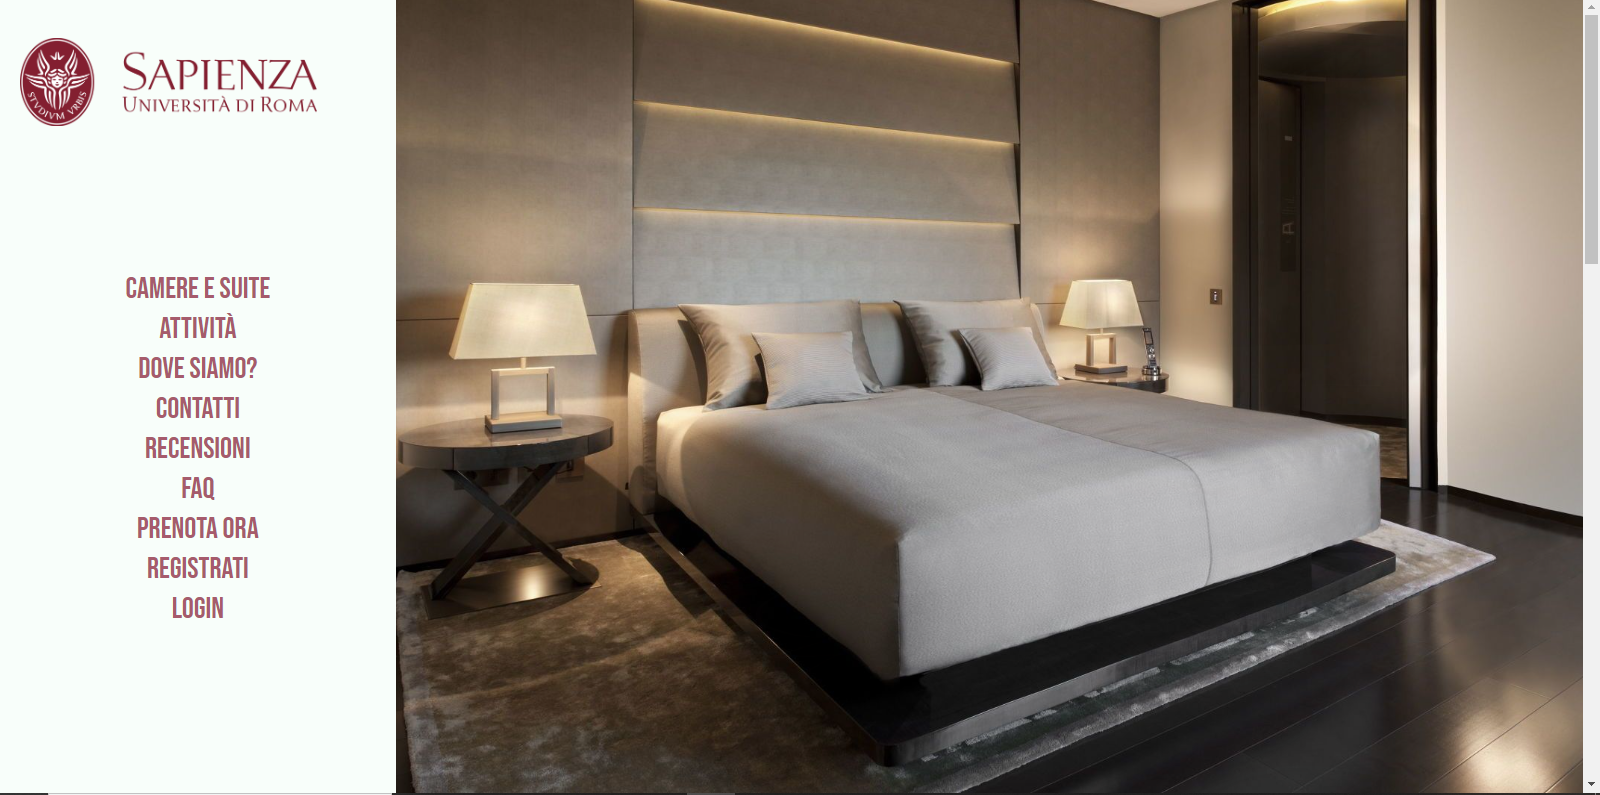
\includegraphics[scale=0.3]{HomePage.png}
\label{intro}
\caption{Homepage del sito}
\end{figure}\\
Tale pagina web è strutturata principalmente in \textbf{due sezioni verticali}, quella di sinistra e di destra. La sezione di destra è composta in \underline{quattro} \underline{sottosezioni orizzontali}: la prima dove vengono mostrate delle \textbf{immagini relative all'hotel} attraverso una animazione a scomparsa ,al di sotto si trovano le restanti sezioni nella quali vengono introdotte le \textbf{attività}, la \textbf{locazione} e i \textbf{contatti} dell'hotel.\\\\
Nella sezione di sinistra troveremo dei link con i quali l’utente potrà interagire cliccandoci sopra. Tra questi se ne possono trovare alcuni unicamente adibiti a scopo informativo che fanno riferimento a sezioni precise della pagina medesima, e sono: 
\begin{itemize}
\item \textbf{Attività:} la quale ci fornisce una piccola introduzione delle varie attività di cui potremmo usufruire avendo un soggiorno attivo.
\item \textbf{Dove siamo?:} fornisce indicazioni sulla locazione della struttura
\item \textbf{Contatti:} fornisce dei contatti di riferimento della struttura. 
\end{itemize}
I restanti link sono: camere e suite,  recensioni, faq, prenota ora, registrati e login. Le funzionalità dell'utente visitatore sono sei principalmente e le andremo ad analizzare più in dettaglio con i relativi link associati.

\medskip

\subsection{Visualizzare le camere e le suite}
\begin{figure}[h]
\centering 
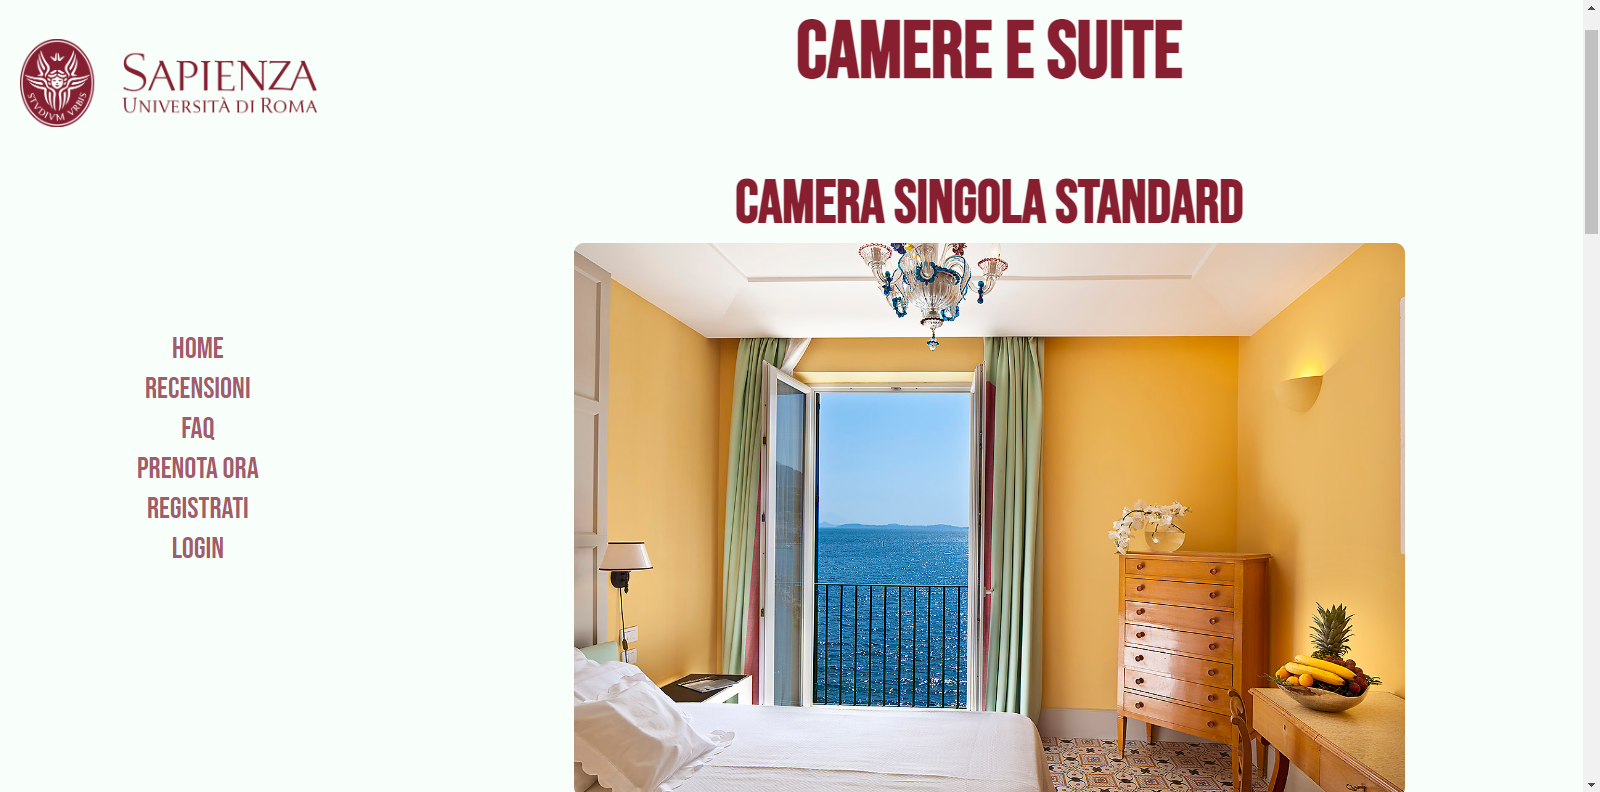
\includegraphics[scale=0.3]{Camere.png}
\caption{Camere e suite}
\label{Camere}
\end{figure}
Cliccando sul link denominato \textbf{"Camere e suite"} nella sezione sinistra della pagina, l'utente verrà indirizzato nella pagina mostrata in figura \ref{Camere}. La struttura della pagina è la stessa della homepage, con piccole differenze. La prima è che nella sezione di destra l'utente potrà prendere coscienza delle camere presenti all'interno della struttura con le relative informazioni associate ad ognuna di esse. La seconda è che nella sezione di sinistra troveremo solamente il link home, per tornare alla pagina principale dell'hotel ed i link delle recensioni, delle faq, della prenotazione di una camera, per la registrazione e per il login. 

\medskip

\subsection{Visualizzare le recensioni}
\begin{figure}[h]
\centering
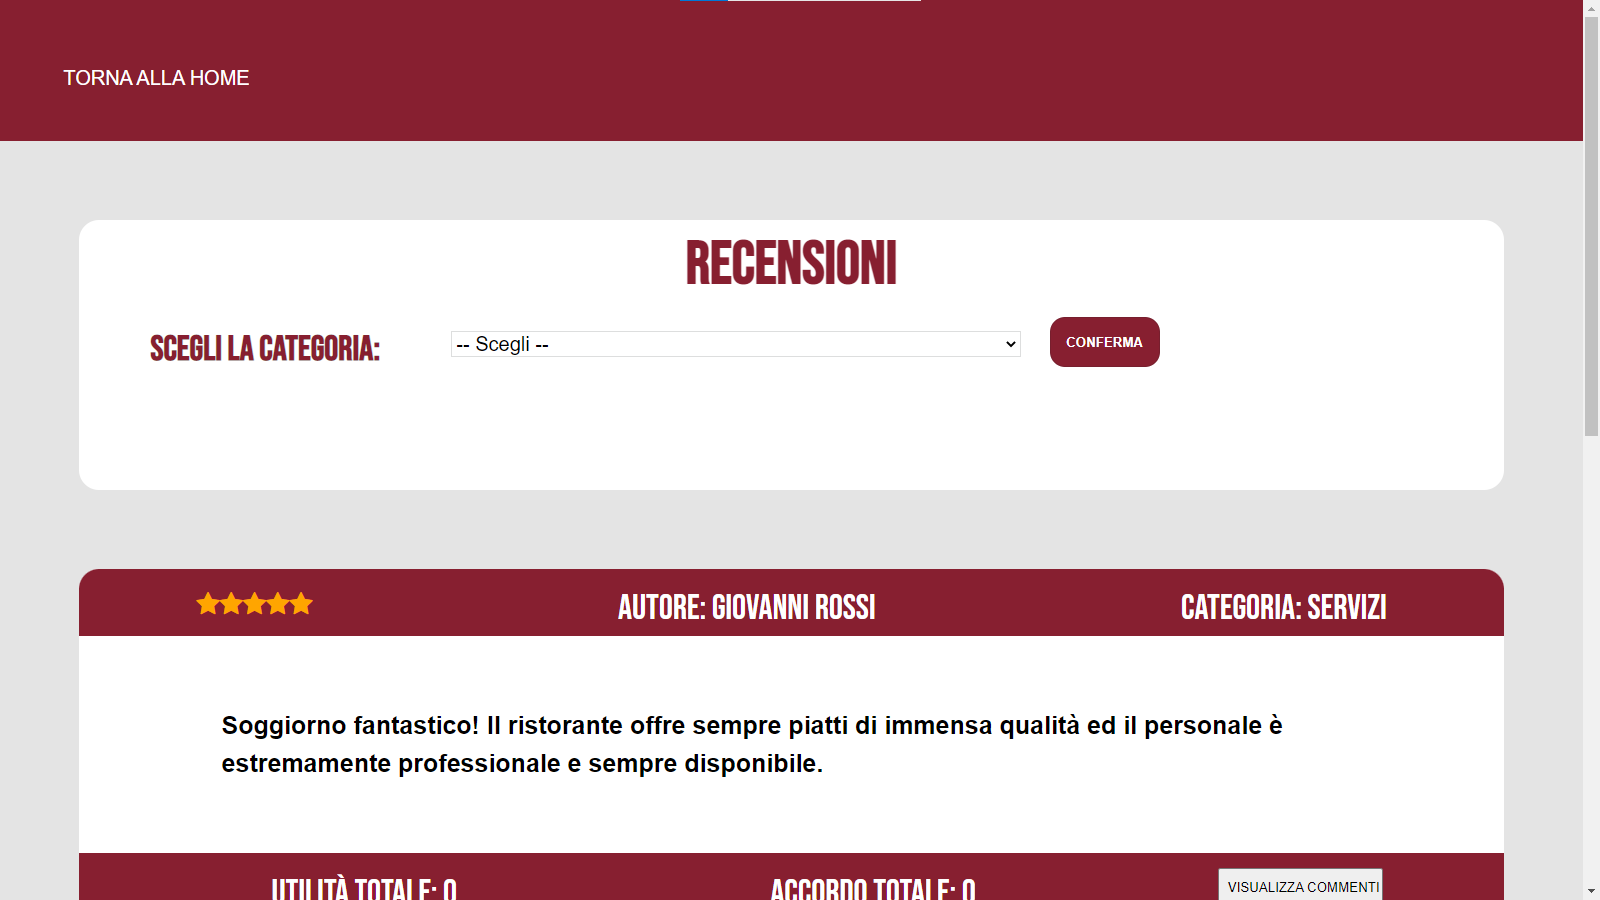
\includegraphics[scale=0.3]{RecensioniVisitatore.png}
\caption{Recensioni - visitatore}
\label{RecensioniVisitatore}
\end{figure}
Interagendo con il link \textbf{"Recensioni"} l'utente si ritroverà nella pagina rappresentata nella figura \ref{RecensioniVisitatore} In questa pagina potrà visionare  tutte le recensioni che sono state scritte dai clienti dell'hotel (cioè tutti utenti registrati all'interno del sito).\\\\
L'utente potrà visionare anche solamente le recensioni delle categorie che più lo interessano andando a selezionare la categoria dal menu a tendina presente nella parte superiore della pagina e andando a cliccare conferma.\\\\
L'utente visitatore avrà anche la possibilità di visualizzare tutti i commenti di risposta di una particolare recensione, andando a selezionare l'apposito pulsante \textbf{"visualizza commenti"} ed essere portato in una pagina come quella mostrata in figura \ref{RisposteRecensioneVisitatore} \newpage
\begin{figure}[h]
\centering
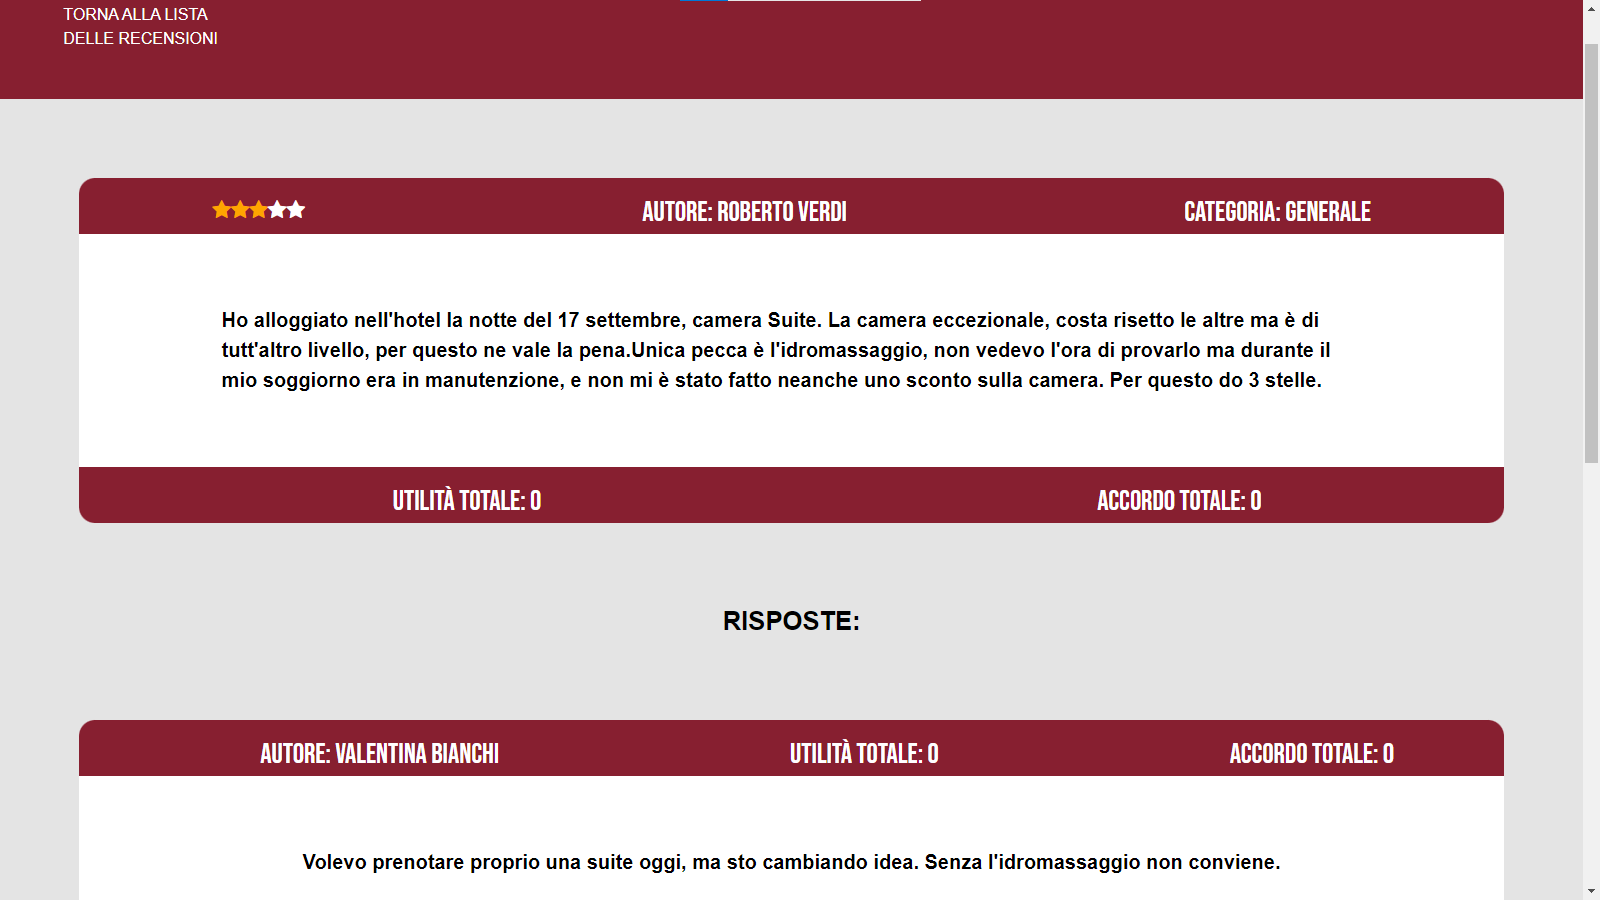
\includegraphics[scale=0.3]{RisposteRecensioneVisitatore.png}
\caption{Commenti di risposta di una recensione - visitatore}
\label{RisposteRecensioneVisitatore}
\end{figure}

\medskip

\subsection{Visualizzare le FAQ}
Nella pagina delle Faq, figura \ref{FaqVisitatore} , accessibile attraverso l'interazione del link presente in home denominato \textbf{"FAQ"}, l'utente è in grado di visionare tutte le Faq dell'hotel che, per definizione, sono delle domande di rilevante importanza e di maggiore frequenza tra l'utenza della piattaforma.
\begin{figure}[!ht]
\centering
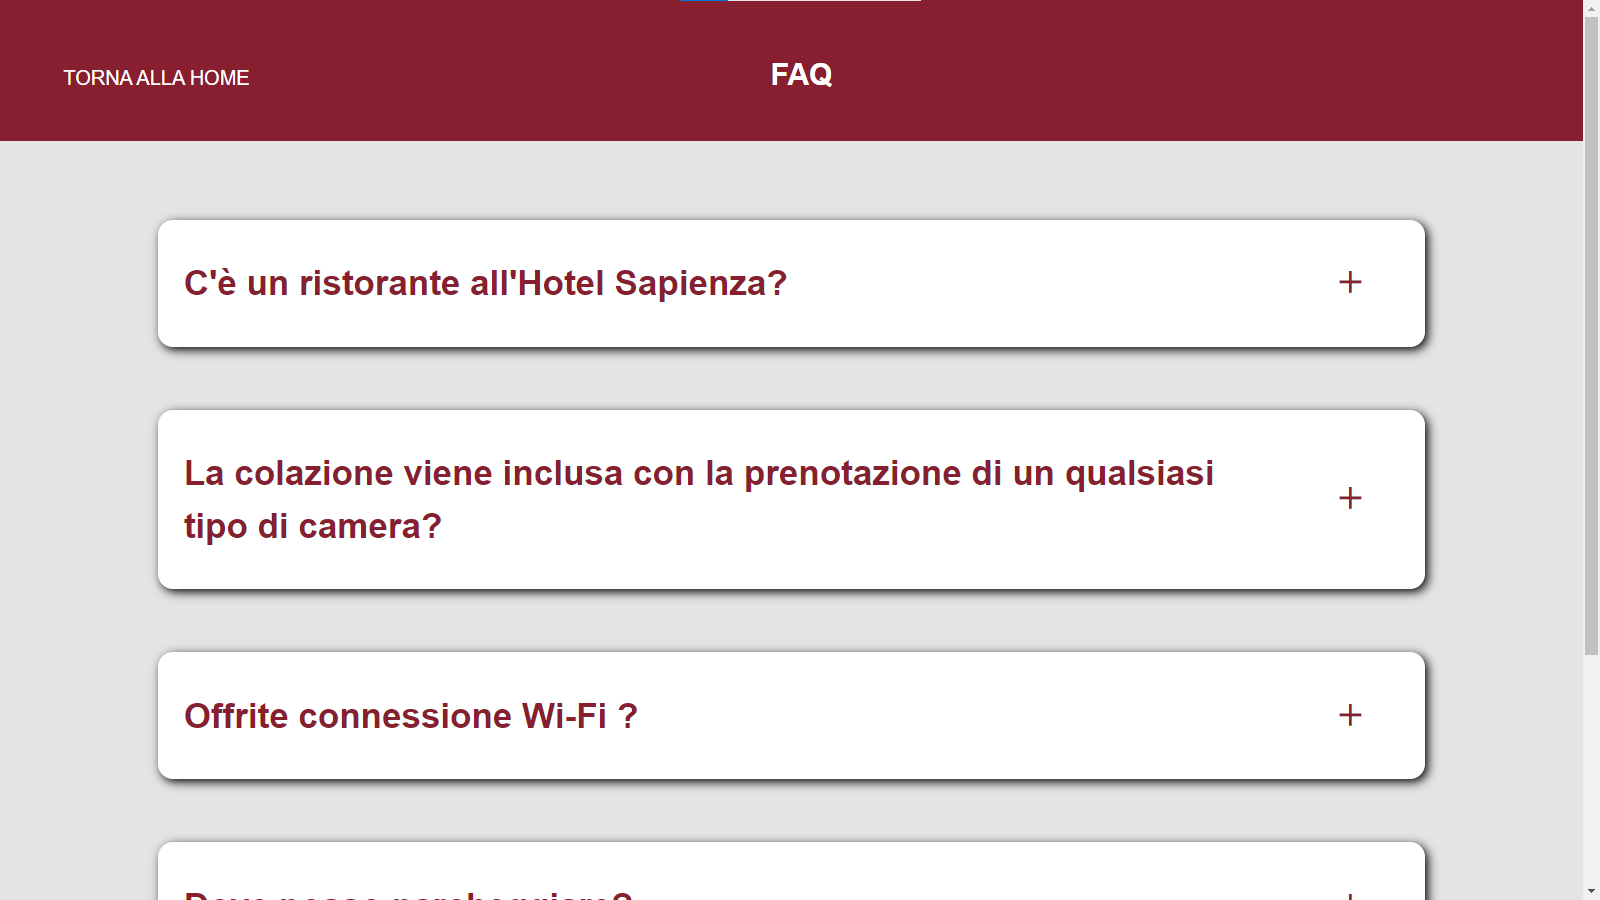
\includegraphics[scale=0.29]{FaqVisitatore.png}
\caption{Pagina delle FAQ}
\label{FaqVisitatore}
\end{figure}

\subsection{Prenotazione di un soggiorno}



\chapter{Programmazione}
In questo capitolo verranno analizzati i vari script che costituiscono il sito web. In particolare, per comodità essi possono essere divisi in due macro-categorie:
\begin{enumerate}
\item \textbf{Script delle pagine:} sono script php contenuti direttamente nelle pagine stesse visualizzate dagli utenti, i cui compiti principali sono: manipolare i dati della pagina, controllare i dati inseriti dall'utente (ed eventualmente della loro correttezza), impostare variabili di sessione, controllare la legalità degli accessi, richiamare gli script delle funzioni ed effettuare il reindirizzamento dell'utente ad altre pagine.
\item \textbf{Script delle funzioni:} essi sono script incapsulati all'interno di funzioni PHP e memorizzati all'interno di appositi file dedicati, non accessibili da nessuna tipologia di utente. Essi sono divisi a loro volta in cinque categorie: 
\begin{enumerate}
\item \textbf{Funzioni Get:} funzioni il cui compito sarà quello di estrarre dati dai file XML ed, in alcuni casi, effettuare dei controlli sui dati estratti.
\item \textbf{Funzioni Modifica:} funzioni il cui compito sarà quello di modificare dei dati già esistenti in un file XML
\item \textbf{Funzioni Insert:} funzioni che andranno ad inserire nuovi dati all'interno di un file XML
\item \textbf{Funzioni delete:} funzioni che andranno a rimuovere dei dati da un file XML
\item \textbf{Funzioni PHP:} funzioni generiche che sono necessarie per il funzionamento del sistema ma non catalogabili in una categoria particolare.
\end{enumerate}
\end{enumerate}

\section{Script delle pagine}
In questa sezione verranno analizzati i vari script contenuti all'interno delle pagine del sito e verrà descritto il loro funzionamento. Per motivi pratici, non verranno esaminate le pagine contenenti esclusivamente script di controllo della legalità dell'accesso


\subsubsection{registrazioneUtente.php}
Lo script contenuto all'interno di questa pagina avrà come scopo principale quello di verificare che l'utente abbia inserito tutti i dati richiesti al momento della registrazione ed, in particolare, della loro correttezza (il codice fiscale deve rispettare un determinato pattern, così come il numero di carta di credito, la mail, ecc..).  Se tutti i dati inseriti sono corretti allora egli passerà a controllare, mediante la chiamata delle funzioni \textit{getCodFisc} e \textit{getUsername}, la presenza di eventuali duplicati del codice fiscale o dell'username inseriti. Se anche quest'ultimi due controlli vanno a buon fine allora si andrà a registrare effettivamente l'utente nel file XML mediante la chiamata della funzione \textit{inserisciNuovoCliente}.

\subsubsection{login.php}
Poiché questa pagina potrà essere aperta in due situazioni differenti (normalmente dalla pagina home oppure automaticamente durante la prenotazione di un soggiorno se l'utente non ha già effettuato il login) il primo scopo di questo script sarà quello di distinguere questi due casi. Ciò viene fatto andando a controllare se la variabile di sessione \textit{prenotazioneCamera} è settata:
\begin{enumerate}
\item In caso negativo, allora verrà visualizzata la normale pagina di login. Dopo aver controllato che l'utente abbia inserito tutti i dati, lo script richiamerà la funzione \textit{eseguiLoginCliente} oppure la funzione \textit{eseguiLoginStaff} dipendentemente da quale tipologia di utente è stata selezionata nella pagina. Se il login del cliente va a buon fine, allora verranno impostate tre variabili di sessione che verranno poi utilizzate dalle altre pagine:
\begin{enumerate}
\item \textit{loginType} (per distinguere il tipo di login che è stato effettuato).
\item \textit{codFiscUtenteLoggato}: verrà passata come parametro ad alcune funzioni presenti nelle varie pagine.
\item \textit{soggiornoAttivo:} memorizza al suo interno la presenza o meno di un soggiorno attivo associato al cliente, cioè con pagamento sospeso oppure con stato \textit{approvato} (un valore \textit{"null"} equivale a dire che il cliente non ha un soggiorno attivo).
\end{enumerate}  
Se invece dovesse andare a buon fine il login del concierge o dell'admin allora sarà sufficiente settare solamente la variabile di sessione \textit{loginType} (il cui valore dipende da quale tipologia di login è stata effettuata).
\item Nel caso in cui la variabile \textit{prenotazioneCamera} dovesse essere settata, allora significa che l'utente stava effettuando la prenotazione di una camera. Dopo aver estratto i dati della prenotazione per poterli salvare in dei campi input \textit{hidden} (in modo da non perderli), verrà visualizzata la normale pagina del login con delle piccole differenze: nella sezione verticale di sinistra verrà visualizzata una sola scritta per annullare la prenotazione in corso e nella sezione di destra non verrà data la possibilità di scegliere il tipo di utente (non si possono associare camere ad utenti registrati come concierge o admin). Il login dopodiché viene svolto normalmente ma con un controllo aggiuntivo: se le credenziali inserite dall'utente sono corrette allora si andrà a controllare, mediante la funzione \textit{getSoggiornoAttivo}, se l'utente che sta effettuando il login ha già un soggiorno attivo. In tal caso, non verrà concesso all'utente di continuare la prenotazione.
\end{enumerate} 

\subsubsection{visualizzaDisponibilita.php}
Questo script andrà prima di tutto a controllare che l'utente sia arrivato in questa pagina in modo legale (cioè inserendo prima delle date in \textit{prenotaOra.php}). Dopodiché, dopo aver estratto dalla variabile di sessione le due date scelte dall'utente, le andrà a passare come parametro alla funzione \textit{getCamereDisponibili}: sulla base del risultato di tale funzione verrà costruita una pagina contenenti tutte le camere che possono essere prenotate nel range temporale inserito dall'utente. Quando l'utente andrà a scegliere una camera, lo script richiamerà la funzione \textit{individuaBottoneCamereDisponibili} per poter individuare quale bottone è stato premuto ed ottenere l'id della camera ad esso associato. Infine, verrà controllato se la variabile di sessione \textit{codFiscUtenteLoggato} è settata: in caso affermativo, allora significa che l'utente ha già effettuato il login e dunque può essere portato nella pagina \textit{confermaPrenotazione.php} per completare la prenotazione. In caso negativo, l'utente verrà portato nella pagina di login.

\subsubsection{confermaPrenotazione.php}
Poiché in questa pagina verranno confermate le prenotazioni di un soggiorno oppure di un'attività, lo script andrà innanzitutto a distinguere quale tipologia di prenotazione l'utente stava effettuando mediante il controllo delle variabili di sessione \textit{prenotazioneCamera} e \textit{prenotazioneAttivita}. Dopo aver estratto i dati necessari che dovranno essere visualizzati all'utente, lo script andrà a costruire una pagina il cui contenuto sarà dipendente dal tipo di variabile di sessione che è stata trovata settata. Se l'utente conferma la prenotazione, allora essa verrà registrata mediante la chiamata della funzione \textit{inserisciPrenotazioneCamera} oppure di \textit{inserisciPrenotazioneAttivita}. Il controllo per capire quale funzione richiamare viene fatto in base a quale input type hidden è stato creato dalla pagina (ad esempio, nel caso della prenotazione di un camera verrà creato un input type hidden  il cui attributo \textit{name} sarà : \textit{idCamera}).

\subsubsection{datiPersonali.php}
Questa pagina potrà essere utilizzata in due circostanze diverse: 
\begin{enumerate}
\item Da un cliente che ha effettuato l'autenticazione e vi accede dalla propria area personale. In tal caso, verrà trovata settata la variabile di sessione \textit{codFiscUtenteLoggato} e dunque verranno estratti i dati personali del cliente mediante la funzione \textit{getDatiCliente} e tutti i soggiorni passati/rifiutati associati a quest'ultimo mediante la funzione \textit{getSoggiorniPassati}
\item Da un admin dopo che ha selezionato un particolare cliente di cui vuole visualizzare (ed eventualmente modificare) i dati personali. In tal caso verranno solamente estratti i dati personali del cliente.
\end{enumerate}
Dopodiché la pagina verrà costruita sulla base dei dati che sono stati estratti

\subsubsection{prenotaTavolo.php}
Il primo passo dello script di questa pagina sarà la definizione della data minima e di quella massima che potranno essere inserite dall'utente per la prenotazione. In particolare:
\begin{enumerate}
\item La data minima viene decisa in base ad un confronto con la data odierna: se quest'ultima è maggiore della data di inizio soggiorno allora la data odierna sarà la minima data che potrà essere scelta. Altrimenti, la data di inizio soggiorno sarà quella minima.
\item La data massima che potrà essere scelta corrisponderà alla data di fine soggiorno.
\item Entrambe le date verranno invertite (cioè verranno scritte nell'ordine \textit{giorno - mese - anno}) in modo tale da renderle idonee per essere impostate come date minime e massime. Tale vincolo viene realizzato andando a passare le variabili php contenenti le date invertite a delle variabili \textit{javascript}. Con quest'ultimo si andrà poi ad impostare un \textit{datePicker} con le date che sono state passate.
\end{enumerate}
Sempre in questa pagina sarà poi presente un campo in cui l'utente potrà scegliere l'orario di prenotazione. Gli orari ammessi per effettuare una prenotazione vengono mostrati in base alla scelta dell'utente del pasto (\textit{pranzo} o \textit{cena}) ed ovviamente sulla base degli orari di apertura e di chiusura del ristorante. Se l'utente ha inserito tutti i dati lo script andrà a richiamare la funzione \textit{cercaTavoloDisponibile} per verificare se è presente o meno un tavolo in grado di soddisfare le richieste del cliente.

\subsubsection{prenotaSC.php}
Lo script di questa pagina andrà a costruire il campo della data e dell'orario per la prenotazione del servizio in camera in modo analogo a quanto detto in \textit{prenotaTavolo.php}. L'unica differenza sarà la presenza di un controllo aggiuntivo riguardante gli orari di modifica del menu: infatti, mediante la funzione \textit{confermaOraUpdateMenu} si andrà a verificare se l'ora corrente si trova all'interno del range orario di modifica del menù. In tal caso non verranno mostrati i campi per inserire la data e l'orario e l'utente non avrà la possibilità di proseguire la prenotazione.







\end{document}